\documentclass[a4paper,12pt]{article}
\usepackage{hyperref}
\usepackage[utf8]{inputenc}
\usepackage[ngerman]{babel}
\usepackage[T1]{fontenc}
\usepackage{amsmath}
\usepackage{amsfonts}
\usepackage{amssymb}
\usepackage{lmodern}
\usepackage[T1]{fontenc}
\usepackage[left=3.5cm,right=2.5cm,top=2.5cm,bottom=2cm]{geometry}
\usepackage[onehalfspacing]{setspace}
\usepackage[backend=biber, doi=true, url=true, sorting=none]{biblatex}
\usepackage{ragged2e}
\usepackage{microtype}
\usepackage{cleveref}
\usepackage{parskip}
\usepackage{graphbox, graphicx}
\usepackage{picinpar}
\usepackage{wrapfig}
\usepackage{tabularx}
\usepackage{isotope}
\usepackage{float}
\usepackage{siunitx}
\usepackage[all]{nowidow}
\usepackage{array}
\usepackage{caption}
\usepackage{csquotes}
\usepackage{newtxtext}
\usepackage{newtxmath}
\usepackage{subcaption}
\usepackage[export]{adjustbox}
\usepackage{multirow}
\usepackage{booktabs}


\addbibresource{BibVerzeichnis.bib}
%*** Command Edits
\newcolumntype{Y}{>{\centering\arraybackslash}X}
\sisetup{output-decimal-marker={,}}
\sisetup{locale = DE}
\DeclareSIUnit\lightyear{ly}
\DeclareSIUnit\parsec{pc}
\DeclareSIUnit\planck{h}
\DeclareSIUnit\speedoflight{c}
\DeclareSIUnit\rplanck{\mathrm{\hslash}}
%\newcommand{\upalpha}{\mathrm{\alpha}}
%\newcommand{\upbeta}{\mathrm{\beta}}
%\newcommand{\upgamma}{\mathrm{\gamma}}



\makeatletter
\renewcommand{\maketitle}{%
Helene-Lange-Gymnasium Fürth
\hfill
Abiturjahrgang 2024/2026 \par
\vskip 3em
\begin{center}
\Huge \textbf{SEMINARARBEIT} \normalsize \par
\vskip 1.5em
Rahmenthema des Wissenschaftspropädeutischen Seminars: \par
\vskip 0.5em
\textbf{\Large Einblicke in die Astronomie} \par
%\vskip 1em
\large Leitfach: \textbf{Physik} \par
\vskip 1em
Thema der Arbeit: 
\vskip -1em
\LARGE \@title \par 
\end{center}
\vskip 3em
\normalsize Verfasser
\hfill
Kursleiter \par 
\large \@author
\hfill
StR Tudor Coldea
\vskip 1em
\large Abgabetermin: 11. November 2025
\vskip 1em
\begin{table}[H]
\begin{tabularx}{\textwidth}{|p{4.3cm}|Y|m{3.8cm}|m{1.3cm}|m{0.5cm}|m{1.3cm}|}
\hline
\textbf{Bewertung} & Note & Notenstufe in Worten & Punkte & & Punkte \\
\hline
schriftliche Arbeit & & & & \center $\times 3$ & \\
\hline
Abschlusspräsentation & & & & \center $\times 1$ & \\
\hline
\multicolumn{5}{r|}{Summe:} &  \\
\cline{6-6}
\multicolumn{5}{r|}{Gesamtleistung nach § 61 (7) GSO = Summe : 2 (gerundet)} & \\
\cline{6-6}
\end{tabularx}
\end{table}
\vfill
\hrule
\footnotesize \textbf{Datum und Unterschrift des Kursleiters} 
\normalsize


  \thispagestyle{empty}
}
\makeatother


\renewcommand\tabularxcolumn[1]{m{#1}}
\renewcommand{\thefigure}{\arabic{figure}}
\newcommand{\figref}[1]{Abb.~\ref{#1}}
\newcommand{\tabref}[1]{Tab.~\ref{#1}}

\crefname{section}{Kapitel}{Kapitel}
\crefname{subsection}{Kapitel}{Kapitel}
\crefname{subsubsection}{Kapitel}{Kapitel}
\Crefname{section}{Kapitel}{Kapitel}
\Crefname{subsection}{Kapitel}{Kapitel}
\Crefname{subsubsection}{Kapitel}{Kapitel}
\crefname{figure}{Abbildung}{Abbildungen}

\DefineBibliographyStrings{ngerman}{
  andothers = {et\addabbrvspace al\adddot}
}



%\renewcommand{\gamma}{\vargamma}
% \DeclareUnicodeCharacter{202F}{FIX ME!!!!}



\begin{document}

\title{\doublespacing {\textbf{VOM GEISTESBLITZ ZUM  \glqq GEISTERTEILCHEN\grqq}}
\vskip 0.6em
 \onehalfspacing \large Über Neutrinos und deren Nutzen für die Wissenschaft am Beispiel des IceCube Neutrino-Detektors}

\author{Nico Schneider}
\date{26. August 2025}
\maketitle

%\onehalfspacing

\newpage
\tableofcontents
\thispagestyle{empty}

\newpage
\setstretch{1.5}
\section{EINLEITUNG} \label{sec:1}
 Was passiert bei einer Supernova? Wie blickt man in das Innere der Sonne? Und was hat ein Eiswürfel mit Astrophysik zu tun?
In Naturwissenschaften stellt man sich ständig Forschungsfragen. Sei es in der Steinzeit, im alten China, im antiken Griechenland oder in der Neuzeit \cite[39, 43, 45--48, 53, 55--56]{Hanslmeier2020} -- schon immer hatte man den Blick dabei auch in den Himmel gerichtet. 
Ob mit optischen Teleskopen oder mit den im 20. Jahrhundert entdeckten nicht-optischen Teleskopen, immer schon nutzte man für die Beobachtung Licht verschiedener Wellenlängen \cite[138, 143]{Hanslmeier2020}. \par
%Die Erfindung des Teleskopes im Jahre 1608 \cite[55]{Hanslmeier2020} war ein großer Fortschritt für die Astronominnen und Astronomen. Es erlaubte viel genauere Beobachtungen, doch auch die Reichweite des Teleskopes ist beschränkt \cite[117]{Hanslmeier2020}. 
%Zu Beginn des 20. Jahrhunderts ermöglichten nicht-optische Teleskope wie Radio- oder Röntgenteleskope wiederum andere Blickwinkel in den Kosmos, da sie jenseits des sichtbaren Lichtes arbeiten \cite[138, 143]{Hanslmeier2020}. \par
Photonen sind dabei ideale Botenteilchen, da sie sich mit Lichtgeschwindigkeit bewegen, sehr klein und neutral geladen sind. Doch auch wenn wir in weit entfernte Galaxien blicken können, lassen uns Photonen nicht in das Innere von Sternen wie unserer Sonne blicken. Sie benötigen mehr als $10^5$ Jahre, um vom Kern an den Rand der Sonne (Photosphäre) zu gelangen, wobei sie ihre Wellenlänge stark verändern \cite[266]{Hanslmeier2020}. Es sollte jedoch auch Teilchen geben, die in nur acht Minuten aus dem Kern der Sonne zur Erde gelangen \cite[266]{Hanslmeier2020}. \par
Diese Teilchen wurden erstmals 1930 erwähnt und heißen Neutrinos. Da sie neutral geladen und fast masselos sind, sind sie nicht durch elektromagnetische Wechselwirkungen und nur geringfügig durch Gravitation beeinflussbar. Ihre Eigenschaften führten dazu, dass man Neutrinos erst 26 Jahre nach ihrer Vorhersage experimentell nachweisen konnte \cite{Cowan1956, Pauli}. Im Gegensatz zu Photonen können Neutrinos viel mehr Materie ungehindert durchdringen und uns deshalb auch aus dem Sonneninneren mit nur acht Minuten Verzögerung erreichen. Seit ihrer Entdeckung spielen Neutrinos in der Astroteilchenphysik eine immer größer werdende Rolle. In Experimenten wie dem IceCube Neutrino-Detektor, einem $\qty{1}{\kilo\cubic\meter}$ großen \glqq Eiswürfel\grqq \ am Südpol, werden Neutrinos aus weit entfernten Galaxien, Supernovae und der Sonne gründlicher denn je untersucht. \cite{UniWisconsin–Madison}. \par
Diese Arbeit soll einen Überblick über die historische Entwicklung der Neutrino-Physik geben und die \glqq Geisterteilchen\grqq \ dabei in das Standardmodell der Elementarteilchen einordnen (\cref{sec:2}). Deren Relevanz für die Forschung soll vor allem anhand des IceCube Neutrino-Detektors nähergebracht werden (\cref{sec:3}). Hauptsächlich wird sich hierbei einer Literaturrecherche bedient, wobei in \cref{ssec:25} mithilfe einer Nebelkammer das Prinzip von Teilchendetektoren experimentell erläutert werden soll.


 

\newpage




\section{GRUNDLAGEN DER NEUTRINO-PHYSIK} \label{sec:2}

\subsection{Über ein Teilchen, das es nicht gibt} \label{ssec:21}

Vor 100 Jahren war es kaum vorstellbar, dass die radioaktiven $\upalpha$-, $\upbeta$- und $\upgamma$-Zerfälle im Unterricht der Mittelstufe behandelt werden \cite{SSB}, da sie damals nur kaum bekannt waren. In den 1910er Jahren untersuchten Wissenschaftlerinnen und Wissenschaftler diese Zerfälle gründlich, nachdem Albert Einstein seine spezielle Relativitätstheorie veröffentlichte. Die Formel $E=m\cdot \mathrm{c}^2$ ermöglichte dafür nämlich neue quantitative Ergebnisse \cite[15]{Close2012}. James Chadwick entdeckte 1914, dass der schon bekannte $\upbeta^-$-Zerfall ($n \rightarrow p + e^-$) scheinbar dem
\begin{figure}[b!]
\centering
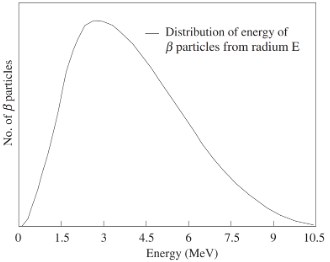
\includegraphics[scale=1]{Betazerfall}
\caption[Kontinuierliches Energiespektrum beim $\upbeta^-$-Zerfall von RaE. -- Quelle: {\cite[][2]{Athar2020}}]{Kontinuierliches Energiespektrum beim $\upbeta^-$-Zerfall von RaE.}
\label{fig:betazerfall}
\end{figure}
wohl wichtigsten Grundsatz der Physik widersprach: der Energieerhaltung \cite[4]{Ecker2020}. Chadwick maß beim $\upbeta^-$-Zerfall (hier beispielsweise von RaE) ein kontinuierliches Energiespektrum der Elektronen \cite[4]{Ecker2020} (vgl. \figref{fig:betazerfall}). Da im Zerfall alle Teilchen neben dem Elektron eine konstante Energie hatten, fragte man sich, wie diese variierende Gesamtenergie zustandekommt. Für den Quantenphysiker Niels Bohr gab es nur eine Möglichkeit, dieses Phänomen zu erklären: Die Energieerhaltung gelte nicht für jeden Zerfall, sondern nur im Mittel \cite[4]{Ecker2020}. Kurz: Er hinterfragte den Energieerhaltungssatz! Der theoretische Physiker Wolfgang Pauli schlug einen anderen, aber ebenfalls radikalen Weg ein. Er postulierte ein Teilchen, das neben dem Elektron beim $\upbeta^-$-Zerfall emittieren würde: Wörtlich schrieb Pauli am 4. Dezember 1930: \glqq Das kontinuierliche beta-Spektrum [sic!] wäre dann verständlich unter der Annahme, dass beim beta-Zerfall [sic!] mit dem Elektron jeweils noch ein Neutron [gemeint war ein Neutrino] emittiert würde derart, dass die Summe der Energien von Neutron und Elektron konstant ist.\grqq \ \cite[2]{Pauli} Pauli ging anfangs noch von einem einzigen neutralen Teilchen aus, darum nannte er dieses eine Teilchen Neutron. \cite[vgl.][2]{Pauli}.
Der Nachweis des neutralen Teilchens war jedoch sehr schwer, weswegen er selbst an seiner Theorie zweifelte: \glqq Ich gebe zu, dass mein Ausweg vielleicht von vornherein wenig wahrscheinlich erscheinen wird, weil man die Neutronen [Neutrinos], wenn sie emittieren, wohl schon längst gesehen hätte.\grqq \ \cite[2]{Pauli} Bohrs Theorie, die Energieerhaltung gelte nicht, konnte nach Messungen widerlegt werden, und Paulis Theorie wurde verfolgt: Enrico Fermi, der auch maßgebend an der Erforschung der Neutrinos beteiligt war, schlug später vor, Paulis \glqq Neutron\grqq \ in ein \glqq Neutrino\grqq \ umzubenennen, da sich entgegen Paulis Erwartung das heute bekannte Neutron von seinem postulierten Teilchen unterscheidet \cite{Fermi1934}. 
Betrachtet man beispielsweise die Zerfallsgleichung 
\begin{equation}
^1_0 \ n \rightarrow ^1_1p +_{-1}^{\hspace{4pt} 0}e + ^0_0 \overline{\nu}_e \text{,}
\label{eq:betaminuszerfall}
\end{equation}
so erkennt man die eminent verschiedenen Massen von Neutron $n$ und (Anti-)Neutrino $\overline{\nu}_e$\footnote{Wie wir noch sehen werden, ist die Masse $m_{\overline{\nu}}$ des Antineutrinos von null verschieden, aber sehr klein ($m_{\overline{\nu}}<\qty[per-mode=symbol]{,45}{\electronvolt\per\square\speedoflight}$) \cite[180]{Aker2025} und unterscheidet sich deutlich von der Masse der Neutronen ($m_n=\qty[per-mode=symbol]{939,56542052(54)}{\mega\electronvolt\per\square\speedoflight} > 2 \cdot 10^9 \ m_{\overline{\nu}}$) \cite[1347]{Tipler2024}. Die $0$ der Zerfallsgleichung bezieht sich lediglich auf die Kernladungszahl des Neutrinos, was dennoch ein großes Indiz für eine geringfügige Neutrino-Masse ist.}.
%Man kann dies unter anderem an den eminent verschiedenen Massen der beiden Teilchen sehen (vgl. \figref{fig:betaminuszerfall}). 
%Auf die Masse und weitere Eigenschaften der Neutrinos wird explizit noch in \cref{ssec:22} eingegangen und soll an dieser Stelle nicht weiter behandelt werden. 
Mit dem Wissen, dass Neutrinos keine Neutronen waren, entstand eine Theorie über die Erforschung der immer noch vermuteten Neutrino-Teilchen. Es stellte sich jedoch heraus, dass eine Messung der Neutrinos, selbst wenn es sie gibt, schier unmöglich ist. Wie sollte man etwas nachweisen, das man quasi nicht messen kann? Erst 1956, also ein Viertel Jahrhundert nach Paulis Postulierung der Teilchen, gelang es Frederick Reines und Clyde Cowan mit viel Arbeit, das Neutrino experimentell nachzuweisen \cite{Cowan1956}. Wie wir in \cref{sssec:221} noch sehen werden, sollte dieses Neutrino nicht das einzige bleiben. Dank ihrer Arbeit an den Neutrinos erhielten Pauli \cite{NPOa}, Fermi \cite{NPOc} und Reines \cite{NPOb} einen Nobelpreis, doch auch Bruno Pontecorvo, der keinen Nobelpreis erhielt, soll an dieser Stelle wegen seiner ehrwürdigen Neutrino-Forschung genannt werden (vgl. \cref{ssec:22}).

\subsection{Die geheimen Facetten des Neutrinos} \label{ssec:22}
\subsubsection{Erst eins, dann zwei, dann drei} \label{sssec:221}
In den 1960ern folgte dem nun Elektron-Neutrino $\nu_e$ genannten Neutrino von Cowan und Reines eine zweite Art von Neutrinos (Myon-Neutrino $\nu_\mu$), das von Lederman, Schwartz und Steinberger entdeckt wurde \cite{NPOd}. Schließlich folgte im Jahr 2000 das Dritte im Bunde: das Tau-Neutrino $\nu_\tau$ \cite{Fermilab} \cite[1--2]{DONUT2001}. Es gibt also verschiedene Arten, die man auch Generationen nennt. Diese drei Neutrino-Generationen gliedern sich in das Standardmodell der Elementarteilchen (vgl. \figref{fig:sm}). 
\begin{figure}[b!]
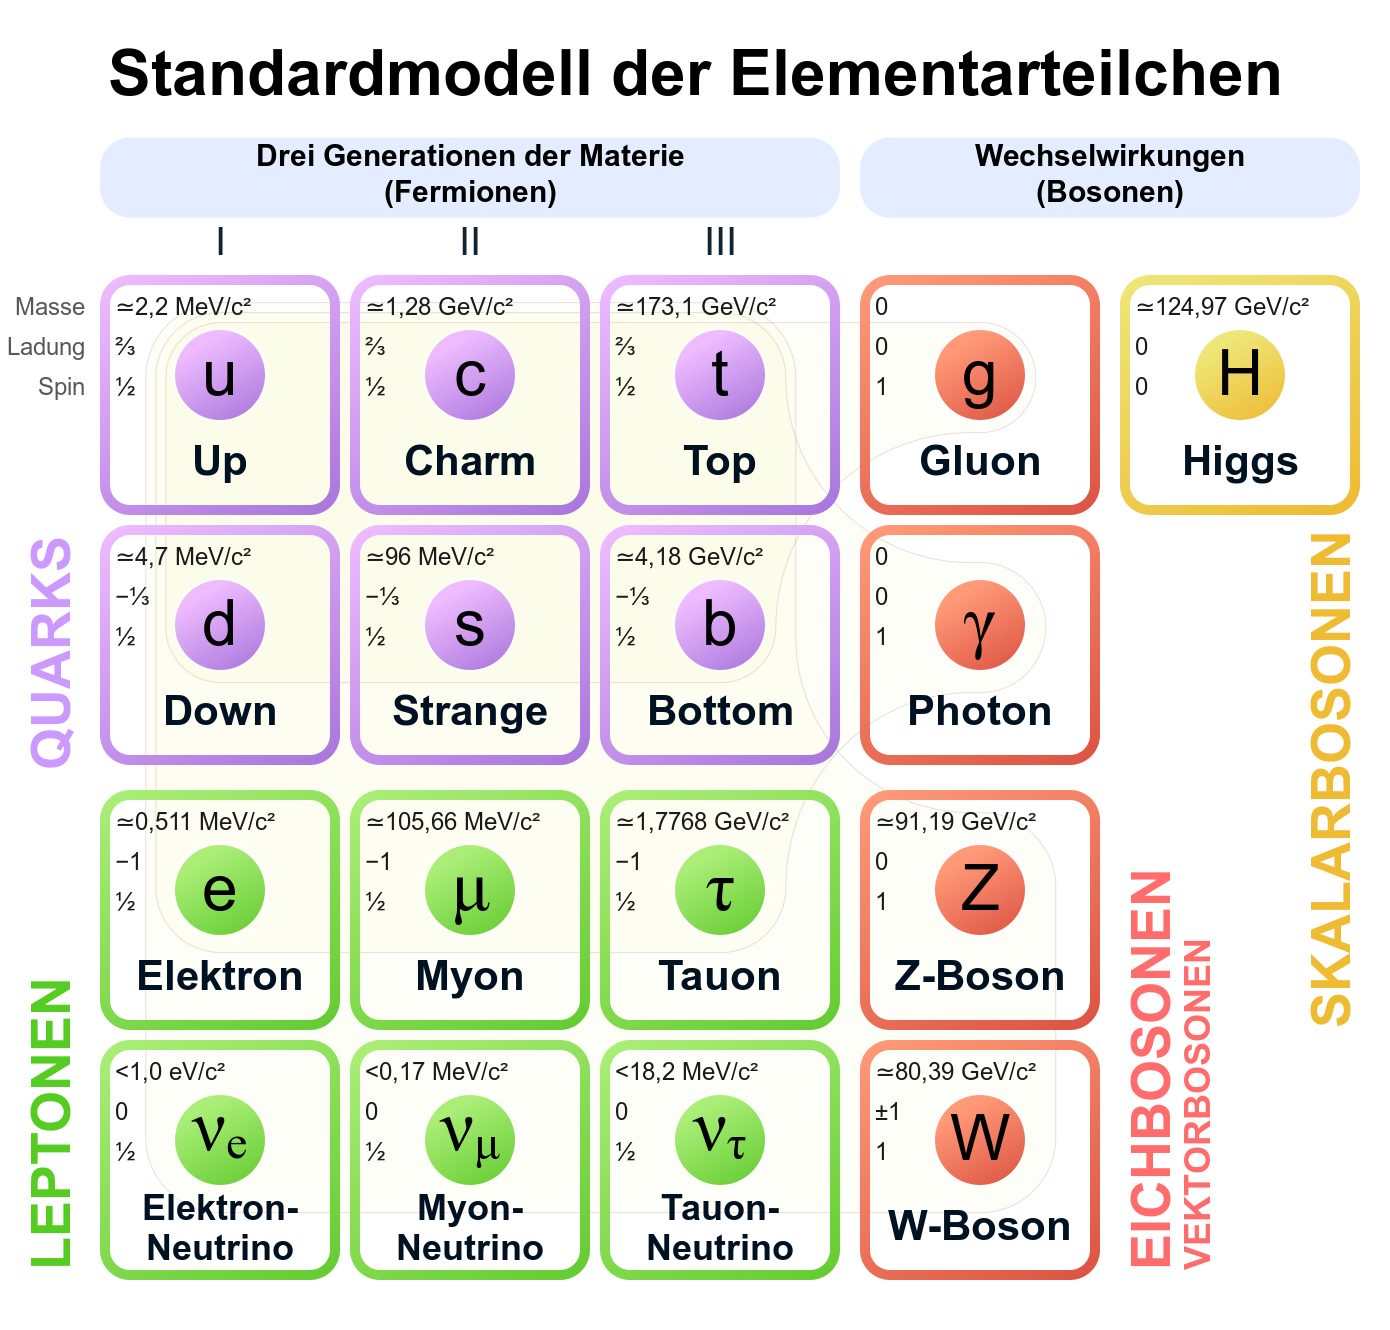
\includegraphics[width=1\textwidth]{Standard_Model_of_Elementary_Particles-de}
\caption[Standardmodell der Elementarteilchen (SM). -- Quelle: Cush via Wikimedia Commons: {\url{https://commons.wikimedia.org/wiki/File:Standard_Model_of_Elementary_Particles-de.svg}} \ (besucht am 31.05.2025).]{Standardmodell der Elementarteilchen (SM).}
\label{fig:sm}
\end{figure}Das Elektron-Neutrino $\nu_e$ ordnet sich unter Up-Quark, Down-Quark und Elektron ein. Man kann sich die zweite und dritte Spalte vereinfacht als \RN{1}. Spalte (Generation) vorstellen, jedoch mit nach rechts hin zunehmender Masse. Wie bei den Quarks auch sind Myon und Tauon schwerere Versionen des Elektron, und so ist es auch bei den Neutrinos. Bei genauerer Betrachtung des SM fällt aber eine Ungewissheit der Neutrinomassen auf. Während bei Quarks und geladenen Leptonen konkrete Massen stehen, sind bei den Neutrino-Generationen nur  Obergrenzen angegeben. Doch wie kommt das? \par
\subsubsection{Über ein \emph{schwieriges} Problem} \label{sssec:222}
Lange Zeit dachte man, Neutrinos seien masselos \cite[26]{Athar2020}, obwohl Wolfgang Pauli 1930 bereits annahm: \glqq Die Masse der Neutronen [gemeint: Neutrinos] müsste von derselben Grössenordnung [sic!] wie die Elektronenmasse sein und jedenfalls nicht grösser [sic!] als $\num{0,01}$ Protonenmasse.\grqq \ \cite[2]{Pauli} Durch Experimente konnte man die Hypothese der von null verschiedenen Masse bestätigen \cite[300]{Zyla2020}. Dennoch ist es schwer, einen konkreten Wert anzugeben, da Neutrinos durch ihre extrem kleine Masse und die neutrale Ladung sehr schwer nachzuweisen sind \cite{Dolan2025}. Heute gibt es laufend Experimente zur Neutrinomasse, die jüngst auch die Grenze aus \figref{fig:sm} verringern konnten. \par 
Das Karlsruhe Tritium Neutrino Experiment (KATRIN) ist im Bereich der direkten Neutrino-Massebestimmung weltweit führend \cite[180]{Aker2025}. Um die Masse von Elektron-Antineutrinos $m_{\overline{\nu}}$ zu messen, wird sich hauptsächlich des $\upbeta$-Zerfalles bedient, wobei KATRIN konkret den Zerfall
\begin{figure}[b!]
\centering
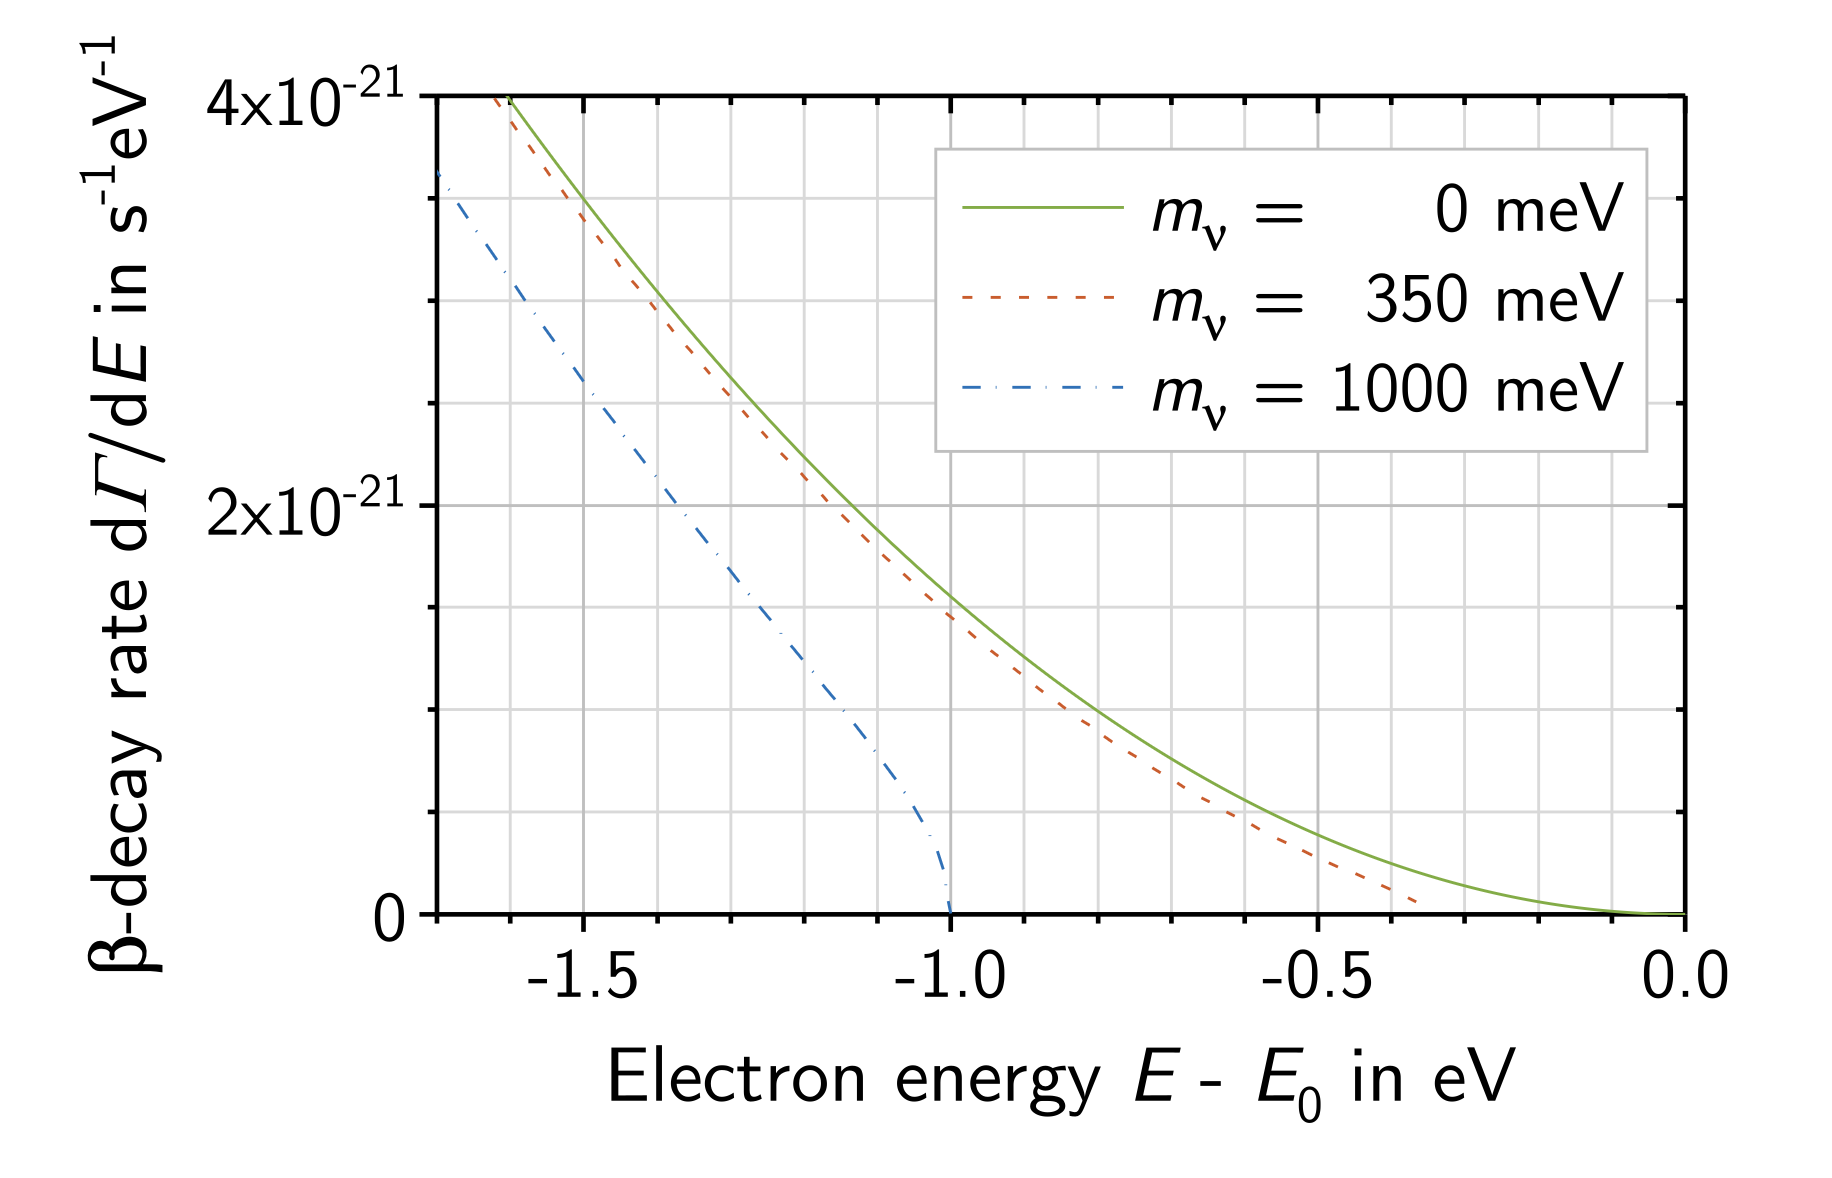
\includegraphics[width=.7\textwidth]{Endpoint}
\caption[Darstellung des differentiellen $\upbeta$-Spektrums nahe $E_0$ unter Annahme verschiedener Neutrino-Massen. -- Quelle: {\cite[][3]{Kleesiek2019}}]{Darstellung des differentiellen $\upbeta$-Spektrums nahe $E_0$ unter Annahme verschiedener Neutrino-Massen.}
\label{fig:endpoint}
\end{figure} 
\begin{equation}
\mathrm{T_2}\rightarrow \isotope[3]{HeT^+} + e^-+\overline{\nu_e}
\label{eq:tritzerfall}
\end{equation}
untersucht \cite[072004-2]{Aker2022}. Um die Schreibweise zu vereinfachen nehmen wir im Folgenden $m_{\nu}=m_{\overline{\nu}}$ an. Mithilfe Fermis Goldener Regel \cite[2]{Kleesiek2019} erkennt man, dass am Endpunkt des $\upbeta$-Spektrums $E_0$, an dem die kinetische Energie $E$ des Elektrons (unter der Annahme von $m_\nu=0$) am höchsten ist, die Kurve des differentiellen $\upbeta$-Zerfall-Spektrums 
\begin{equation}
R_{\upbeta}(E;E_0,m_\nu^2)\;\propto\;(E_0 - E)\,\sqrt{(E_0 - E)^2 - m_\nu^2} \hspace{1em}\text{\cite[180]{Aker2025}}
\label{eq:diffspec}
\end{equation}
am meisten verzerrt wird (vgl. \figref{fig:endpoint}). $R_{\upbeta}(E;E_0,m_\nu^2)$ ist hierbei die differentielle Spektrumsrate (auch als $\frac{\mathrm{d}\Gamma}{\mathrm{d}E}$ bezeichnet), also die Anzahl an Zerfällen pro Sekunde pro Energie \cite[2--3]{Kleesiek2019}. $E_0$ liegt im übrigen stets am energiereichen Rand des Spektrums, der sich in \figref{fig:betazerfall} beispielsweise circa bei $E_0\approx \qty{10,5}{\mega\electronvolt}$ befindet. Ziel von KATRIN ist es, in genau diesem Spektrum nahe $E_0$ fein zu messen, um eine Obergrenze zu finden \cite[180]{Aker2025}.
\par
Das $\qty{70}{\meter}$ lange Experiment gliedert sich in sechs Teile (vgl. \figref{fig:katrin}), wobei die Überwachung und Steuerung in Abschnitt (a) geschieht \cite[6]{Kleesiek2019}. In Abschnitt (b) werden die $\upbeta^-$-Zerfälle durch das Tritium nach Zerfall (\ref{eq:tritzerfall}) erzeugt, die dann auf einer magnetischen Bahn (c) mit $B=\qty{2507}{\tesla} \pm \qty{,25}{\percent}$ \cite[180]{Aker2025} in Richtung eines Vor-Spektrometers (d) geleitet werden \cite[6]{Kleesiek2019}. Dabei wirkt das Vor-Spektrometer als eine Art Hochpassfilter, das nur Elektronen mit Energien nahe des Endpunkts $E_0=\qty{18,57}{\kilo\electronvolt}$ der Art $E\geq (E_0- \qty{300}{\electronvolt})$ passieren lässt \cite[1--3]{Prall2012}. Im Haupt-Spektrometer (e) selbst können die gesuchten Neutrinos nahe des Endpunktes $E_0$ in Energiefilter mit Bandbreiten bis zu $\qty{2,0}{\electronvolt}$ sortiert werden \cite[181]{Aker2025}. Abschnitt (f) detektiert zuletzt die passierenden Elektronen aus (e) mit bis zu $\qty{95}{\percent}$ Effizienz \cite[181]{Aker2025}. \par
So schaffte es die KATRIN Collaboration im April 2025, die Obergrenze für Elektron-Antineutrinos von $<\qty[per-mode=symbol]{,8}{\electronvolt\per\square\speedoflight}$ auf $<\qty[per-mode=symbol]{,45}{\electronvolt\per\square\speedoflight}$ mit $\qty{90}{\percent}$ Sicherheit zu drücken \cite[180]{Aker2025}.
\begin{figure}[b!]
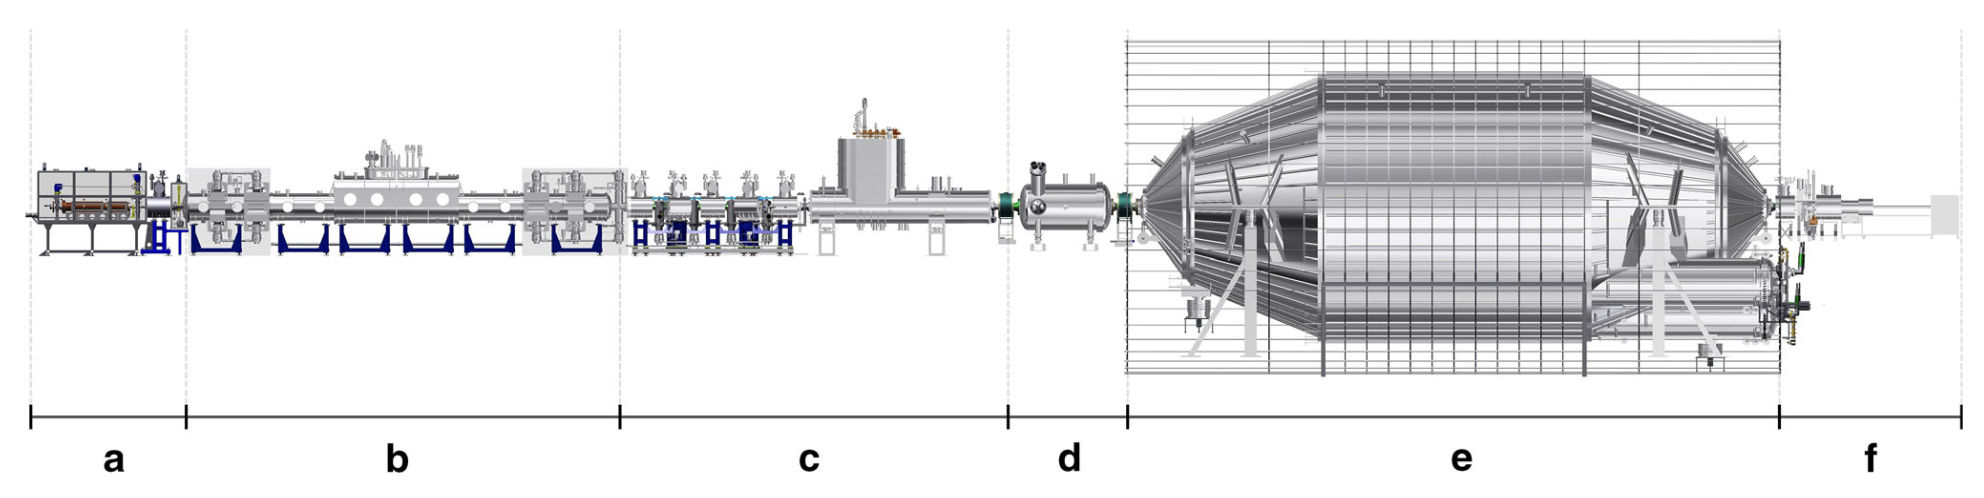
\includegraphics[width=\textwidth]{KATRIN}
\caption[Aufbau des KATRIN-Experiments. -- Quelle: {\cite[][6]{Kleesiek2019}}]{Aufbau des KATRIN-Experiments.}
\label{fig:katrin}
\end{figure}

\subsubsection{Geschmäcker sind verschieden -- oder?} \label{sssec:223}
Nachdem die zweite Generation von Neutrinos entdeckt wurde, verfasste der bereits in \cref{ssec:21} erwähnte Bruno Pontecorvo mit Wladimir Gibrow 1969 einen Aufsatz über die Theorie, dass Neutrinos in ihre Antiteilchen übergehen können \cite{Bilenky2014}. Sie gingen in Analogie von neutralen Kaonen davon aus, dass der Zustand der in schwachen Wechselwirkungen erzeugten Neutrinos eine Superposition von Neutrino $\nu$ und Antineutrino $\overline{\nu}$ ist \cite[10]{Athar2022}. Später formulierten Maki, Nakagawa und Sakata die Vermutung, dass Neutrinos in ihrer Generation oszillieren können \cite[870--871]{Maki1962}. Damals war das $\tau$-Neutrino noch nicht entdeckt, weshalb es in ihrem Artikel keine Erwähnung fand. Diese sogenannte Flavor-Oszillation der Neutrinos lässt sich aber problemlos auf die dritte Generation erweitern. Dabei ist jedes erzeugte Neutrino eine Art Superposition der Zustände aller drei Neutrino-Generationen \cite[10]{Athar2022}. Jeder der drei Zustände $m_1$, $m_2$, $m_3$ besitzt dabei eine eigene Masse, wobei die Voraussetzung für die Oszillation nun ist, dass bei $n$ Eigenzuständen $(n-1)$ Zustände eine von null verschiedene Masse haben \cite[10]{Athar2022}. \par 
Die Erforschung der Neutrinos ist sein sehr theoretisches Feld, in dem sich mehrere Varianten und Hypothesen zu Neutrinos gebildet haben. Im Folgenden sollen die grundlegenden Eigenschaften von zwei dieser Modelle vorgestellt werden. \par
\subsubsection{Dirac-Neutrinos} \label{sssec:224}

\begin{table}[b!]
%\renewcommand{\arraystretch}{1.2}
\centering
\begin{tabular}{p{4cm} >{\centering\arraybackslash} p{1.6cm} >{\centering\arraybackslash} p{2cm} >{\raggedleft\arraybackslash}p{1.6cm}}
%\toprule
Name  					& Teilchen							& Ladung in $e$& Spin in $\unit{\rplanck}$ \\
\midrule
Elektron-Neutrino		&$\nu_e$							&						&\multirow{3}{*}{$+\dfrac{1}{2}$} \\
%\cmidrule{1-2}
Myon-Neutrino			&$\nu_\mu$							&$0$					&								\\
%\cmidrule{1-2}       
Tauon-Neutrino 			&$\nu_\tau$							&						&	\\
\midrule         
Elektron-Antineutrino	&$\overline{\nu}_e$					&						&\multirow{3}{*}{$-\dfrac{1}{2}$}   \\
%\cmidrule{1-2}
Myon-Antineutrino		&$\overline{\nu}_\mu$				&$0$						&								\\
%\cmidrule{1-2}
Tauon-Antineutrino		&$\overline{\nu}_\tau$				&						&									\\
\midrule
Elektron				&$e^-$								&						&\multirow{3}{*}{$+\dfrac{1}{2}$}  \\
%\cmidrule{1-2}
Myon					&$\mu^-$							&$-1$					&									\\
%\cmidrule{1-2}
Tauon					&$\tau^-$							&						&									\\
\midrule
Positron				&$e^+$								&						&\multirow{3}{*}{$-\dfrac{1}{2}$}  \\
%\cmidrule{1-2}	
Anti-Myon				&$\mu^+$							&$+1$					&								\\
%\cmidrule{1-2}
Anti-Tauon				&$\tau^+$							&						&									\\
\bottomrule
\end{tabular}
\caption[Teilchen-Antiteilchen-Beziehung der Leptonen. -- Quelle: Autor.]{Teilchen-Antiteilchen-Beziehung der Leptonen nach dem SM.}
\label{tab:lepton}
\end{table}

Im (erweiterten) Standardmodell der Elementarteilchen \cite[vgl.][285--286]{Zyla2020} werden Neutrinos als Fermionen aufgefasst, die neben sich selbst auch ein Antiteilchen haben (vgl. \tabref{tab:lepton}). Da Neutrinos neutral geladen sind, unterscheiden sie sich von ihren Antiteilchen durch Spin und Leptonenzahl, nicht aber in ihrer Ladung \cite[13]{Athar2022}. Der Spin kann als eine Art innerer Drehimpuls von Teilchen angesehen werden. Frank Close erklärt in seinem Buch \glqq Neutrinos\grqq : \glqq Die Quantentheorie zeigt, dass [der Spin] nur bestimmte Werte annehmen kann, die entweder ungeradzahlige oder geradzahlige Vielfache einer gewissen Grundeinheit sind. Aus historischen Gründen ist diese Grundeinheit des Spins $1/2$ [$\mathrm{\hslash}$].\grqq \ \cite[29]{Close2012}. Die Quarks und Leptonen, die allesamt den Spin $\qty[parse-numbers=false]{\frac{1}{2}}{\rplanck}$ haben, bilden die Gruppe der Fermionen (benannt nach Enrico Fermi). Aus dieser Teilchengruppe besteht Materie. \unit{\rplanck} ist hierbei die reduzierte Planck-Konstante $\qty{1}{\rplanck} = \frac{\unit{\planck}}{2\uppi} = \num{1,054571817}\ldots\cdot 10^{-34} \ \unit{\joule\second}$ \cite[1347]{Tipler2024}. Zur Verdeutlichung der Leptonenzahl werden mithilfe der Schreibweise für Dirac-Neutrinos (nach Paul Dirac) die zwei Neutrino-Zustände
\begin{equation}
\nu^D_{l+} \text{ bzw. } \overline{\nu}^D_{l-}
\label{eq:diracneutrino}
\end{equation}   
eingeführt \cite[13]{Athar2022} \cite[23--25]{Athar2020}. 
\begin{table}[b!]
\centering
\renewcommand{\arraystretch}{1.2}
\begin{tabularx}{.7\textwidth}{YYY}
%\toprule
Spin in $\unit{\rplanck}$ & Neutrino & Anti-Neutrino \\
 \midrule
$+ \dfrac{1}{2}$ & $\nu^D_{l+}$ & $\overline{\nu}^D_{l+}$ \\
\addlinespace
$- \dfrac{1}{2}$& $\nu^D_{l-}$ & $\overline{\nu}^D_{l-}$ \\
\bottomrule
\end{tabularx}
\caption[Darstellung der vier Dirac-Zustände eines Neutrinos. -- Quelle: Autor.]{Darstellung der vier Dirac-Zustände eines Neutrinos.}
\label{tab:dirac}
\renewcommand{\arraystretch}{1}
\end{table} Hierbei ist $D$ die Kennzeichnung der Neutrinos als Dirac-Neutrinos (im Unterschied zu Majorana-Neutrinos $\nu^M$). Das $l$ ist die Leptonenzahl, wobei $\nu^D_{l}$ immer $L_l=+1$ und $\overline{\nu}^D_{l}$ immer die Leptonenzahl $L_l=-1$ zugeordnet wird \cite[13]{Athar2022}. Es soll erwähnt sein, dass die Operatoren $+$ und $-$ im Index der Schreibweise (\ref{eq:diracneutrino}) keine Aussage über die Leptonenzahl geben, sondern dem Neutrino den Spin $+ \frac{1}{2} \ \hslash$ bzw. $- \frac{1}{2} \ \hslash$ zuordnen \cite[13]{Athar2022}. \par 
Grundsatz im SM ist weiterhin, dass die Leptonenzahl stets erhalten bleibt \cite[285]{Zyla2020}. Mithilfe der eingeführten Schreibweise für Dirac-Neutrinos und der Einführung der Leptonenzahl lassen sich nicht nur zwei, sondern vier unterschiedliche Zustände von Neutrinos gleicher Masse konstruieren (vgl. \tabref{tab:dirac}). Diese vier unterscheidbaren Zustände werden als Dirac-Neutrinos bezeichnet \cite[13]{Athar2022} \cite[23--25]{Athar2020}.
%Dirac-Neutrinos besitzen aber nicht nur diese zwei Zustände, sondern auch die unterscheidbaren Zustände $\nu^D_{l+}$ und $\overline{\nu}^D_{l-}$ \cite[13]{Athar2022}. $\nu^D_{l+}$ unterscheidet sich von $\nu^D_{l-}$ durch den anderen Spin, während $\nu^D_{l-}$ nämlich linksdrehend den Spin $-\frac{1}{2} \ \hslash$ aufweist, ist $\nu^D_{l+}$ rechtsdrehend mit Spin $+\frac{1}{2} \ \hslash$. Bei $\overline{\nu}^D_{l-}$ ist ebenfalls der Spin genau entgegengesetzt des Anti-Neutrinos $\overline{\nu}^D_{l+}$. 

\subsubsection{Majorana-Neutrinos} \label{sssec:225}
Anders als in \cref{sssec:224} werden Majorana-Neutrinos $\nu^M$ (nach Ettore Majorana) als Neutrinos mit einzig zwei Zuständen aufgefasst \cite[24]{Athar2020}. Neutrinos wären dann ihre eigenen Antiteilchen $\nu^M=\overline{\nu}^M$ \cite[286]{Zyla2020}. Diese andere Auffassung der Neutrinos hätte eine weitreichende Konsequenz \cite[25]{Athar2020}. \par
Prämisse im SM ist, dass die Leptonenzahl erhalten bleibt. Bei einem $\upbeta^-$-Zerfall nach $n \rightarrow p + e^-$ hätte man allerdings einen Widerspruch erzeugt, da auf der rechten Seite der Gleichung ein Lepton vorhanden ist, damit also $L=1$ ist, wobei auf der linken Seite nur das Neutron (kein Lepton) mit Leptonenzahl $L=0$ ist\footnote{Auf eine Differenzierung der Leptonenzahl nach ihrer Generation wird an dieser Stelle verzichtet. Es wird im Folgenden also anstelle der Einelbetrachtungen von $L_e$, $L_\mu$ und $L_\tau$ nur die Summe der drei Leptonenzahlen der Art $L=L_e+L_\mu+L_\tau$ betrachtet.}. Heute ist der Zerfall allerdings mit Neutrinos erklärbar. Es gilt für $\upbeta$-Zerfälle
\begin{table}[H]
\begin{tabularx}{\textwidth}{p{1.0cm} X}
 & $n \rightarrow p + e^- + \overline{\nu_{e}}$ \\
 und & $p \rightarrow n + e^+ + \nu_{e}$,
\end{tabularx}
\end{table}  
wobei sich die Leptonenzahl rechts jeweils durch Teilchen und Antiteilchen neutralisieren (Neutron und Proton sind keine Leptonen, somit gilt links stets $L=0$). Für die Leptonen bei diesem Zerfall ist $L=+1$ und für die Antiteilchen der Leptonen $L=-1$, wobei man durch Addition der Leptonenzahlen den Endzustand $L=-1+1=0$ erhält. Offenbar reicht das SM aus, um diese Zerfälle zu erklären, da hier die Leptonenzahl links und rechts der Zerfallsgleichung übereinstimmt. Doch Majorana-Neutrinos ermöglichen einen \emph{neutrinolosen doppelten $\beta$-Zerfall} der Art
\begin{equation}
n + n \rightarrow p + p + e^- + e^- \text{,}
\end{equation}
wobei sich die Neutrinos der beiden einzelnen $\upbeta^-$-Zerfälle durch $\nu^M = \overline{\nu}^M$ auslöschen würden. Die Erhaltung der Leptonenzahl wäre nicht gegeben, da eine Differenz der von zwei Einheiten entstünde. Das SM hätte dafür keine Erklärung. \par
Es ist keineswegs einfach, zu erforschen, ob Neutrinos nun Dirac- oder Majorana-Neutrinos sind. Es wird viel Motivation in die Beantwortung dieser Frage gesteckt, da sie unsere Weltvorstellung verändern könnte \cite{Cirigliano2022}\cite{Balantekin2019}. Diese Arbeit bezieht sich, wenn nicht anders gekennzeichnet, auf Dirac-Neutrinos und deren Eigenschaften. \par

\subsection{Der Blick ins Universum} \label{ssec:23}

Neutrinos spielen für die Astrophysik eine große Rolle. Anfänglich wurden Neutrinos vor allem zur Erforschung der Sonne genutzt, was auch zum sogenannten \glqq Solar Neutrino Problem\grqq \ führte. Raymond Davis Jr. et al. hatten Neutrinos von der Sonne messen wollen, jedoch lag die Neutrino-Rate ca. $\frac{2}{3}$ unter dem erwarteten Wert \cite[1205]{Davis1968}. Dieses Rätsel wurde dann mithilfe der Neutrinooszillation gelöst: Viele der von ihnen erwarteten Neutrinos hatten ihre Generationen in eine gewandelt, die der Detektor nicht messen kann \cite[213--214]{Suzuki2000}. \par
Später wurde die erste von Messinstrumenten aufgezeichnete Supernova, die Supernova 1987A, mit Neutrinoteleskopen untersucht. Gleich drei Teleskope konnten Neutrinos von dieser Supernova nachweisen \cite{Aglietta1987, Bionta1987, Hirata1987}. So konnte man unter anderem herausfinden, dass Supernovae die stärksten bekannten Quellen für Neutrinos sind \cite[23]{Janka2011}. Seitdem gab es keine weitere bekannte Supernova, wodurch sich im Bereich der Supernovae-Beobachtungen seit 1987 nichts verändert hat. \par
Wie auch in \cref{ssec:32} noch ersichtlich wird, liegt die Stärke der Neutrinos in der großen Reichweite, die sie zurücklegen können, ohne ihren Informationsgehalt zu verlieren. Sie können ihre Richtung und damit ihren Ursprung auch auf weiten Strecken noch zuverlässig übermitteln. Geladene Teilchen können magnetisch abgelenkt werden, auch Photonen fallen dieser Wechselwirkung zum Opfer. Auf langen Distanzen sind Neutrinos also bessere Boten als Photonen, was sie für die Erforschung von weit entfernten Galaxien obligat macht. 

\subsection{Das Unsichtbare sichtbar machen} \label{ssec:24}

Wie bereits in \cref{ssec:21} ersichtlich wurde dauerte es lange, bis man von der Existenz von Neutrinos überzeugt war. Die Kombination aus neutraler Ladung und sehr geringer Masse machen eine Wechselwirkung mit anderen Teilchen, und damit den Nachweis von Neutrinos selbst, nämlich sehr kompliziert. Es war zuallererst Bruno Pontecorvo, der einen Vorschlag zum Nachweis der Neutrinos machte. Er schlug 1946 vor, einen großen Tank voll Chlor zu nehmen und dort Umwandlungsprozesse, angestoßen durch von Uran emittierte Neutrinos, zu detektieren. Das Chlor würde sich bei der Neutrino-Wechselwirkung in Argon der Art $\mathrm{\nu}_e+ \isotope[37]{Cl} \rightarrow \upbeta^- + \isotope[37]{Ar}$ \cite[697]{Kolanoski2016} umwandeln und dabei $\upbeta^-$-Strahlung emittieren \cite[1--5]{Pontecorvo1946}.
\begin{figure}[b!]
\centering
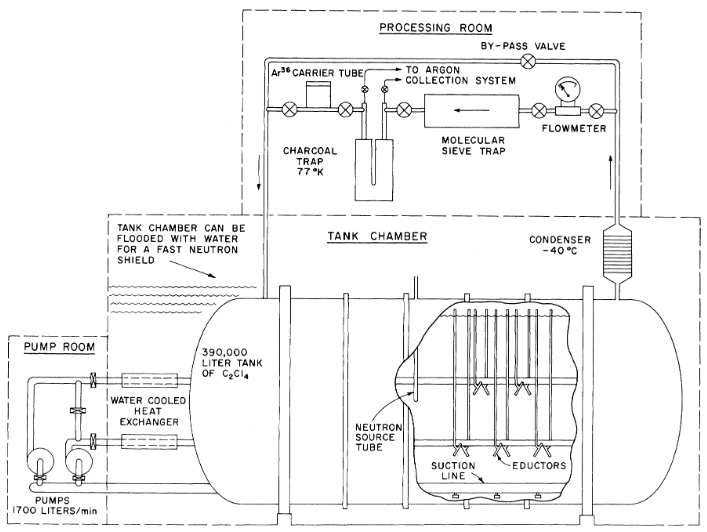
\includegraphics[width=0.7\textwidth]{Davis_Aufbau}
\caption[Aufbau des Experiments von Davis. -- Quelle: {\cite[][1206]{Davis1968}}]{Aufbau des Experiments von Davis.}
\label{fig:davis}
\end{figure} \par
Nun brauchte es noch einen Wissenschaftler, der dieses Experiment auch umsetzen würde. Raymond Davis wurde 1914 in Washington D.C. geboren und war von klein auf für Chemie begeistert \cite[22]{Lande2009}. 1942 erwarb er den Doktortitel in Chemie und ging 1948 schließlich zum neuen Brookhaven National Laboratory, das für den friedlichen Einsatz von Kernenergie forschte \cite{NPO}. Er selbst forschte an Neutrino-Nachweisen und führte das von Pontecorvo vorgeschlagene Experiment durch (vgl. \figref{fig:davis}), konnte aber zu seiner Überraschung keine signifikanten Ergebnisse erzielen \cite{NPO}.
Was er und auch Pontecorvo nämlich nicht wussten ist, dass es nicht Neutrinos waren, die das Uran erzeugte, sondern Antineutrinos. \par
1956 gelang C. L. Cowan und Fred Reines der Nachweis der Neutrinos, was Reines 1995 schließlich den Nobelpreis einbrachte \cite{Cowan1956, NPOb}. Zwar bauten sie wie Davis einen großen Detektor, jedoch wiesen sie keine Element-Umwandlungen nach, sondern Gamma-Strahlen, die von inversen $\upbeta^+$-Zerfällen ($\overline{\nu}_e + p \rightarrow n + \upbeta^+ + \upgamma$) erzeugt wurden \cite{Cowan1956}. \par
Seither gibt es viele verschiedene Arten, Neutrinos zu detektieren, und eine Art ist die Nutzung des Cherenkov-Effekts (benannt nach Pavel A. Cherenkov): \glqq Durchquert ein geladenes Teilchen mit einer Geschwindigkeit $v$ ein Medium mit dem Brechungsindex $n$ und ist die Geschwindigkeit größer als die Phasengeschwindigkeit des Lichts im Medium $c_n$ [...], so wird elektromagnetische Strahlung emittiert. [$c_n= \frac{\mathrm{c_0}}{n}$,  $\mathrm{c_0}$: Lichtgeschwindigkeit im Vakuum]“ \cite[437]{Kolanoski2016} Wie bei einem Überschallflugzeug, an dem sich Kondensstreifen bilden, entsteht hier ein Schwall an blauem Licht, der hinter den geladenen Teilchen abstrahlt (vgl. \figref{fig:cherenkov}).
\begin{figure}[t!]
\centering
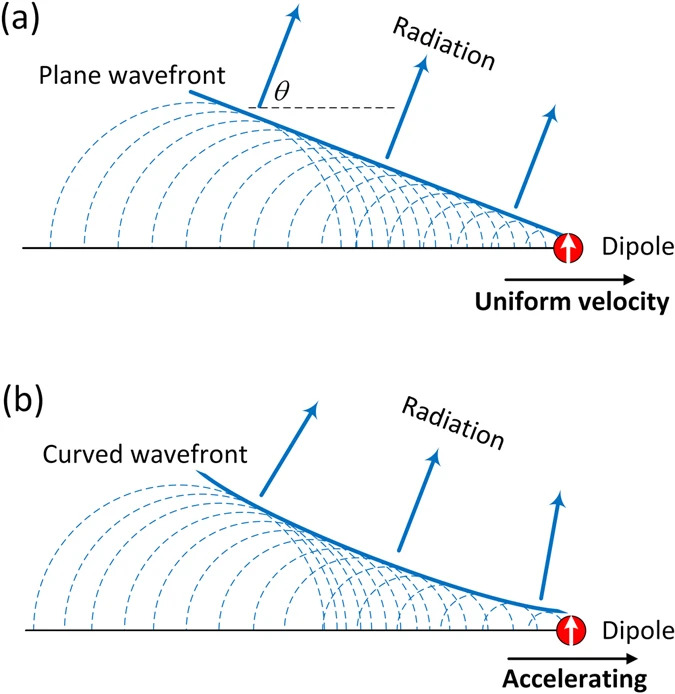
\includegraphics[width=0.6\textwidth, trim={0 410pt 0 0}, clip]{cherenkov}
\caption[Cherenkov-Effekt: Der Dipol löst einen Schwall an blauem Licht aus. (Bearbeitet durch den Autor.) -- Quelle: {\cite[][2]{Hu2017}}.]{Cherenkov-Effekt: Der Dipol löst einen Schwall an blauem Licht aus. (Bearbeitet durch den Autor.)}
\label{fig:cherenkov}
\end{figure} \par
Cherenkov-Strahlung, die Methode von Cowan et al. als auch alle anderen Nachweismethoden von Neutrinos haben eines gemeinsam: Sie weisen nie direkt Neutrinos nach. Durch ihre Eigenschaften lassen sich Neutrinos nur indirekt, also durch Wechselwirkung mit anderen Teilchen, nachweisen. Beim Cherenkov-Effekt müssen Neutrinos erst wechselwirken, sodass geladene Teilchen entstehen, denn sie selbst sind neutral geladen und damit nicht in der Lage, die Cherenkov-Strahlung zu emittieren.

\subsection{Auf den Spuren der Teilchennachweise: Ein Experiment} \label{ssec:25}

Um die theoretischen Ideen der Teilchendetektion praxisnah und anschaulich zu präsentieren, wurde für diese W-Seminararbeit ein Experiment durchgeführt. In der sog. Nebelkammer wurde 1932 das Positron \cite{Anderson1933} und 1937 das Myon nachgewiesen \cite{Street1937}.
\begin{center}
\large Experiment: Teilchennachweis in einer Nebelkammer \\
\small Nico Schneider, Yannik Stecher, Tudor Coldea, Hans Wirsching, Lena Pfeifer
\end{center} 
\normalsize 04. Juli 2025
\hfill
Helene-Lange-Gymnasium Fürth, n010



\subsubsection{Ziel und physikalische Grundlagen} \label{sssec:251}

Um genauer zu verstehen, wie Teilchendetektoren funktionieren, soll dieses Experiment der Veranschaulichung dienen. Wir wollen, auch unter Zunahme von radioaktiven Präparaten, Teilchenspuren von $\upalpha$- und $\upbeta$-Strahlung sichtbar machen und auch die kosmische Hintergrundstrahlung der Myonen untersuchen. \par
Die Nebelkammer funktioniert nach einem einfachen Prinzip: In einem durchsichtigen Gehäuse ist die Atmosphäre mit Alkohol gesättigt. Am oberen Ende des Gehäuses wird Alkohol verdampft während selbiger an der Bodenplatte wieder kondensiert. Durch die Kühlung entsteht ein Temperaturgefälle, wodurch der Alkohol bis zu wenigen Centimetern über der Bodenplatte überkritisch ist. Das hat zur Folge, dass ionisierende Strahlen Tröpfchen des Alkohols auskondensieren und eine Nebelspur sichtbar wird. Aus Länge, Dicke und Form der Spur lassen sich Rückschlüsse auf Teilchenart und kinetische Energie ziehen \cite[166--167]{Kolanoski2016}.

\subsubsection{Versuchsaufbau} \label{sssec:252}



Der Aufbau ist analog zu \cref{sssec:251} gehalten (vgl. \figref{fig:versuchsaufbau}): Im durchgeführten Versuch wird als Alkohol Isopropanol (Propan-2-ol) verwendet. Als durchsichtige Box wird eine transparente Box der Bauart \glqq SAMLA\grqq \ verwendet \cite{IDGK}. Auf ihrem Boden wird ein in Isopropanol getränkter Filz mit Magneten befestigt, der der Verdampfung des Alkohols dient (vgl. \figref{fig:samla}). Es wird ein größenverstellbares Backblech gewählt, das in Länge und Breite mit der Grundfläche der Box übereinstimmt. Die Kühlung erfolgt mittels Trockeneis. Um eine großflächige Auflage des Bleches mit dem Trockeneis zu gewährleisten, wird das Styroporgefäß, in dem das Trockeneis geliefert wird, an zwei Seiten aufgeschnitten (vgl. \figref{fig:trockeneis}). Die Seiten der SAMLA-Box werden mit Plastilin abgedichtet, um ein geschlossenes System anzustreben (vgl. \figref{fig:abdichtung}). Die Durchführung erfolgt in einem abgedunkelten Raum, um die Spuren durch das Licht einer Taschenlampe sichtbar zu machen, da bei Tageslicht keine Spuren sichtbar werden. Im späteren Verlauf werden erst radioaktive $\upbeta$-Strahler an die Box gehalten, anschließend wird ein Loch gebohrt, um einen $\upalpha$-Strahler auf den Versuch strahlen zu lassen. Auf Schutz- und Vorsichtsmaßnahmen wird hinreichend wertgelegt (vgl. \figref{fig:radiosafety}).
\begin{figure}[t!]
\centering
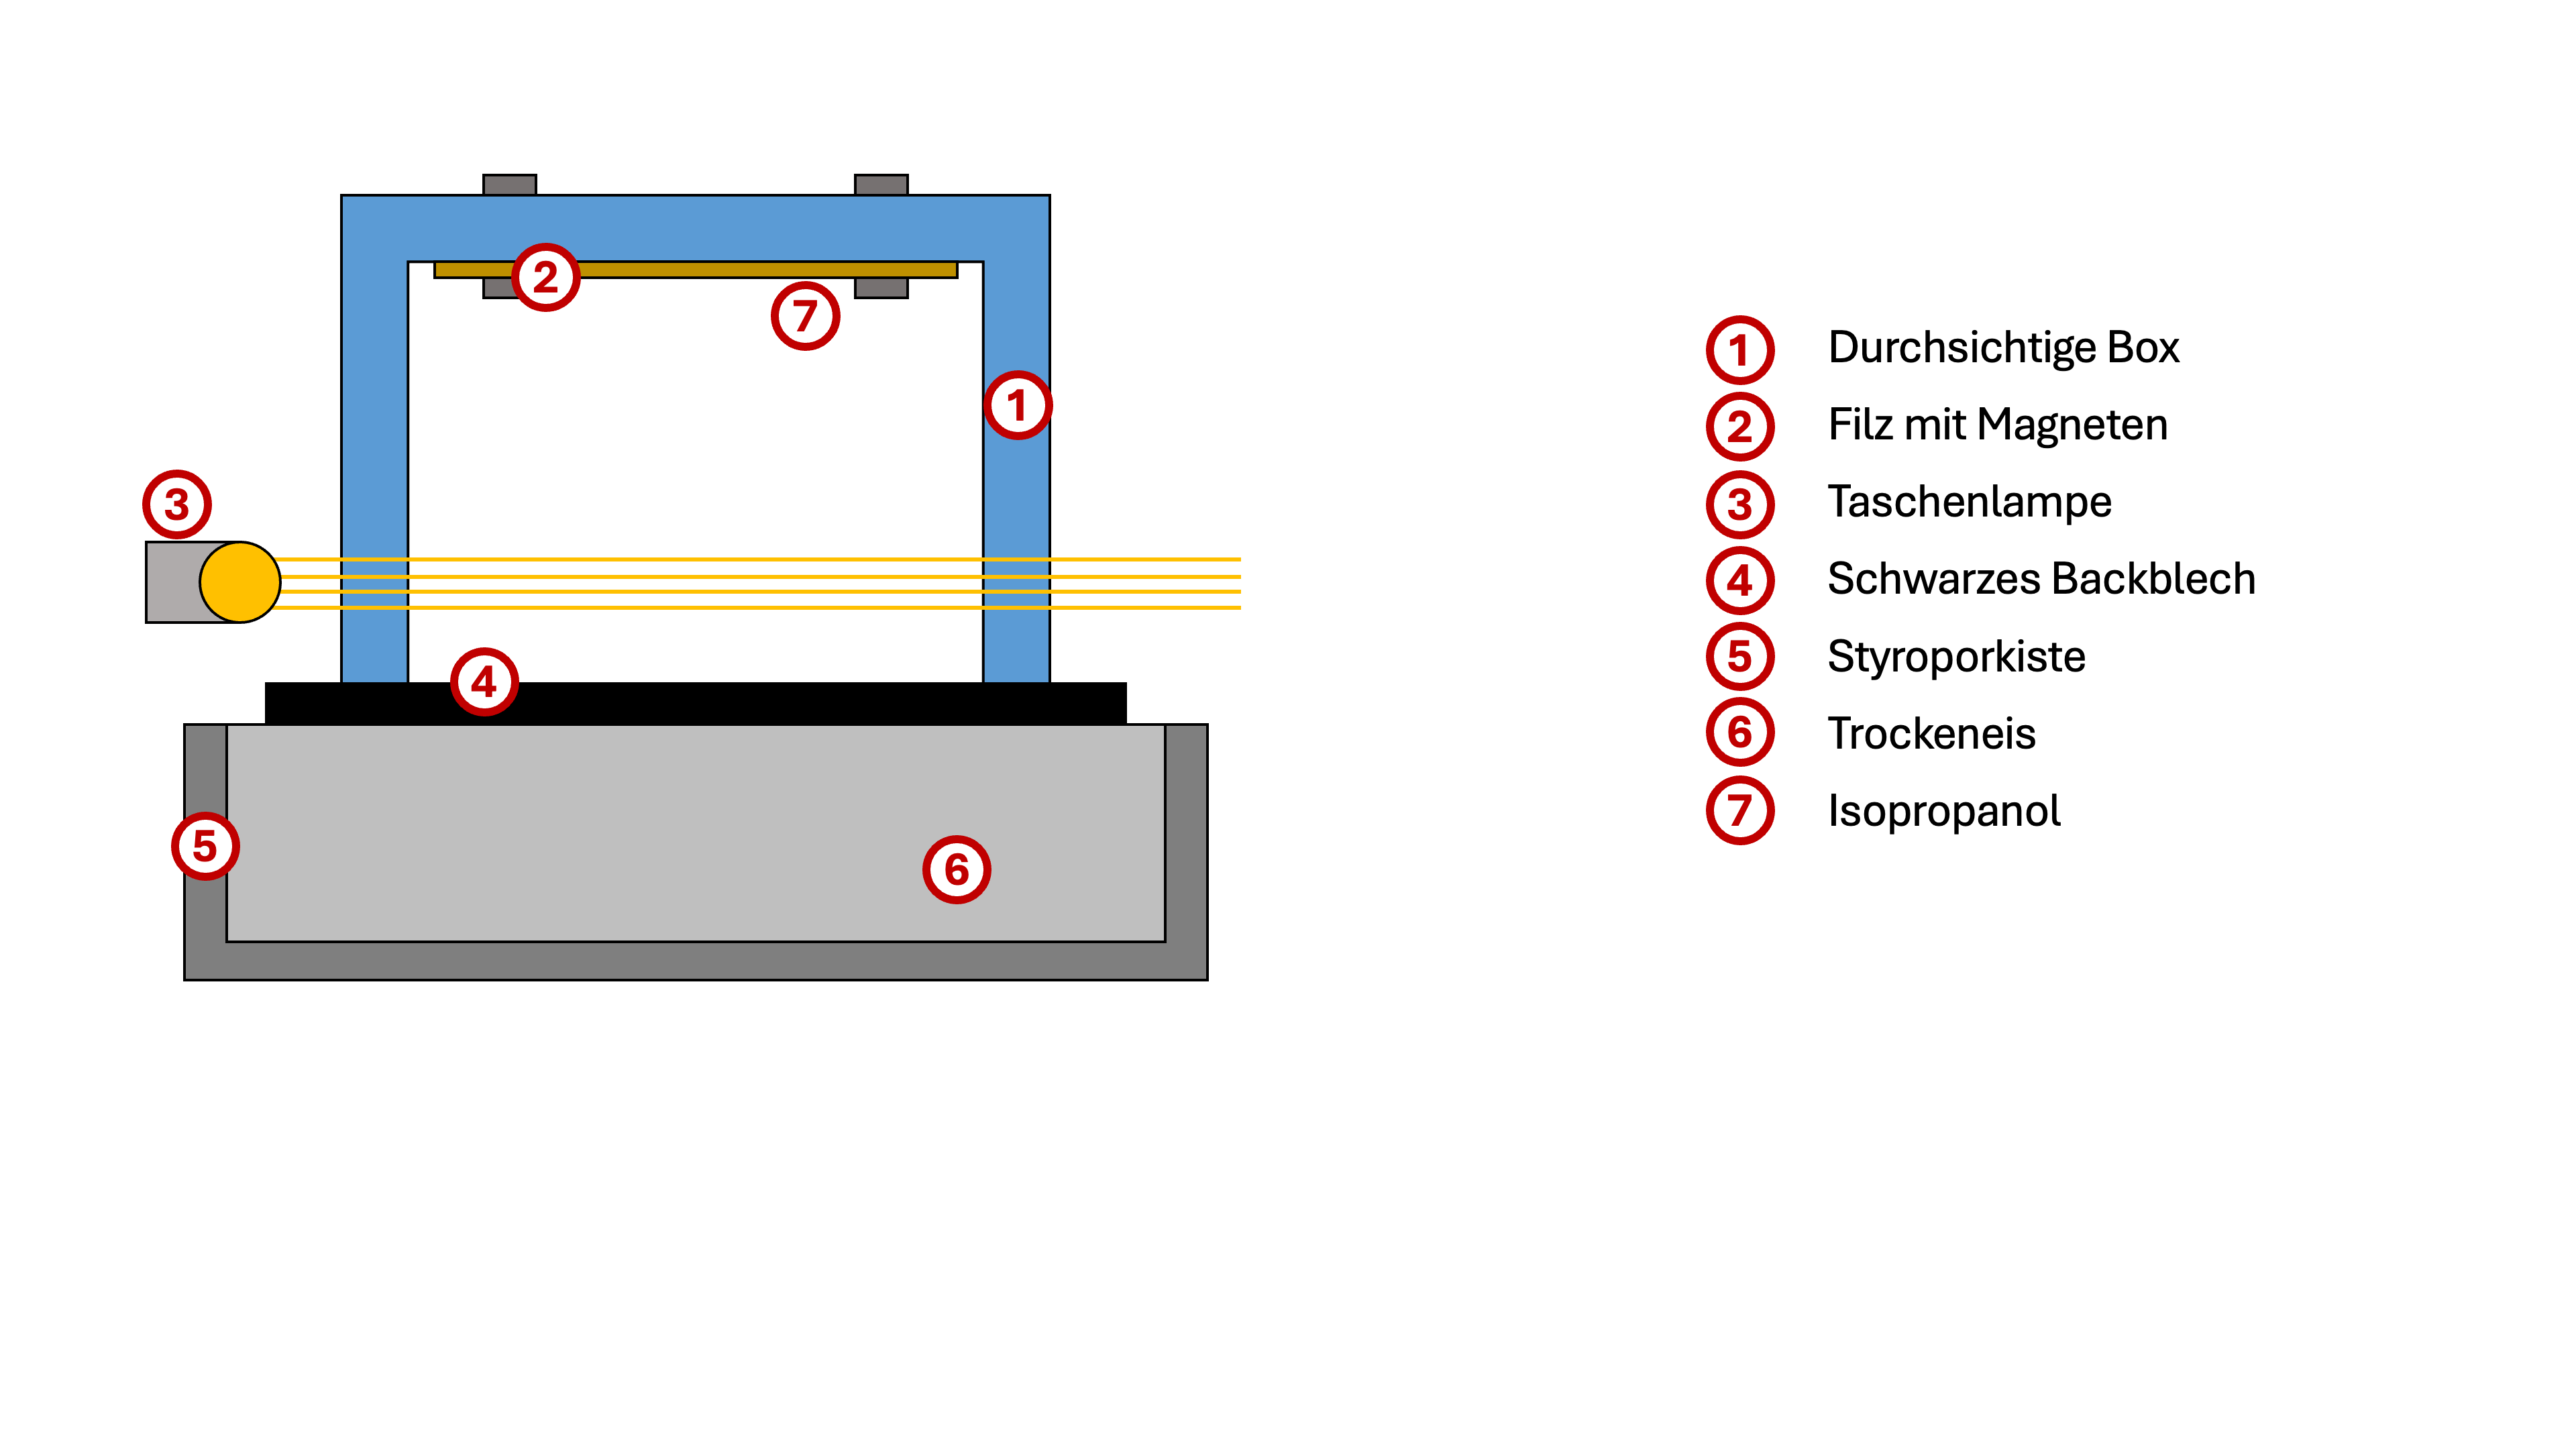
\includegraphics[width=\textwidth, trim={0 160pt 0 60pt}, clip]{Versuchsaufbau_2}
\caption[Versuchsaufbau, nicht maßstabsgetreu. -- Quelle: Autor. ]{Versuchsaufbau, nicht maßstabsgetreu.}
\label{fig:versuchsaufbau}
\end{figure}



\subsubsection{Beobachtungen} \label{sssec:253}

Ohne radioaktive Präparate lässt sich ein gewisses Grundrauschen an kondensiertem Isopropanol beobachten. Keine signifikante Häufung an Spuren ist vorzufinden (vgl. \figref{fig:grundrauschen}). \par
Mit Zuhilfenahme von radioaktiven Präparaten lassen sich erste erkennbare Spuren beobachten. Mittels einer aus Uran bestehenden Armbanduhr, die als $\upbeta$-Strahler wirkt, können Spuren aufgenommen werden, die sich als dünne, gekrümmte Spuren charakterisieren lassen (vgl. \figref{fig:elektron}). Andere Spuren sind länger und deutlicher sichtbar (vgl. \figref{fig:myon}). Bei Verwendung eines anderen $\upbeta$-Strahlers (Sr-90) ist der Spurenteppich dem der Armbanduhr ähnlich. \par
Unter Verwendung des $\upalpha$-Strahlers Ra-226 (Aufbau vgl. \figref{fig:taschenlampe}) können zudem kurze und dicke Spuren aufgenommen werden (vgl. \figref{fig:alpha}). \par
Eine ungewöhnliche Entdeckung ist ein Knick in einer Spur eines Teilchens. Nach einer geraden Strecke \glqq knickt\grqq \ die Spur um ca. $\qty{90}{\degree}$ und streckt sich dann weiter geradlinig durch den Nebel, wenngleich die Spur nach diesem Knick dünner wirkt (vgl. \figref{fig:knick}). \par
Die Spuren entstehen allesamt langsam genug, dass das menschliche Auge den Entstehungsprozess nachverfolgen kann. 



\subsubsection{Auswertung} \label{sssec:254}

Ohne radioaktive Präparate kann nur Hintergrundstrahlung in die Nebelkammer eindringen. Diese Strahlung ist aber sehr geringfügig, weshalb man dort nur wenige Spuren finden kann. \par
Hält man einen $\upbeta$-Strahler an die Wand der Nebelkammer, so dringen $\upbeta$-Teilchen, also Elektronen oder Positronen, in die Nebelkammer ein. Sie sind als längliche, dünne Spuren erkennbar \cite[167]{Kolanoski2016}. Die $\upbeta$-Teilchen mit Ladung $\pm 1$ polarisieren das Isopropanol, und es kommt zur Kondensation der Isopropanol-Teilchen (siehe \cref{sssec:251}). (Anti-)Myonen sind ebenfalls Leptonen mit Ladung $\pm 1$, was ihnen und ihren Spuren ähnliche Eigenschaften wie den $\upbeta$-Teilchen zuschreibt. Durch die größere Masse sind sie energetischer als das leichte Pendant, was in Verbindung mit der gleichen Größe eine längere Spur ermöglicht. In \figref{fig:myon} kann man die Spur also einem Myon zuordnen \cite[vgl.][167]{Kolanoski2016}. \par
Um jedoch $\alpha$-Teilchen in die Nebelkammer eindringen zu lassen, genügt es nicht, die $\alpha$-Quelle nur an die Wand zu halten. Denn $\alpha$-Teilchen haben nur eine sehr geringe Durchdringungsfähigkeit \cite[80]{Stolz2005}. Durch die Bohrung eines Loches wird jedoch den Eintritt in die Nebelkammer ermöglicht (\figref{fig:alpha}). Die kurzen und dicken Spuren sind charakteristisch für $\alpha$-Teilchen, da sie eine deutlich größere Masse im Vergleich zu $\upbeta$-Teilchen haben ($\mathrm{m_\upalpha} \approx 7300 \cdot \mathrm{m_\upbeta}$) \cite[51]{C.C.Buchner2012}. Sie werden durch Reibung wegen ihrer Größe stark gebremst, wodurch die Spur nicht annähernd so lang wie bei anderen Teilchen ist \cite[vgl.][167]{Kolanoski2016}. \par
Bei der Spur mit dem Knick könnte es sich um einen Myonen-Zerfall handeln, bei dem ein Myon in ein $\upbeta$-Teilchen und unsichtbare Neutrinos zerfällt, jedoch stellt Prof. Dr. Anna Nelles in einer E-Mail fest: \glqq Es gibt unglaublich viele Teilchenreaktionen, die ihr [sic!] Teilchen erklären könnten.\grqq \ [A. Nelles, persönliche Kommunikation, 21. August 2025] Somit ist die Spur durchaus außergewöhnlich, aber nicht eindeutig bestimmbar. \par
Unter Rückbezug auf die Ziele aus \cref{sssec:251} lässt sich feststellen, dass die Funktionsweise eines Teilchendetektors erläutert wurde und Myonen beobachtet werden konnten. Die Ziele des Experimentes wurden also allesamt erreicht. 

\begin{table}
	\begin{minipage}[t]{0.48\textwidth}
	\adjincludegraphics[width=\textwidth, clip, valign=t]{Grundrauschen_scaled}
	\captionof{figure}[Grundrauschen. -- Quelle: Autor.]{Grundrauschen.}
	\label{fig:grundrauschen}
	\end{minipage} \hfill
	\begin{minipage}[t]{0.48\textwidth}
	\adjincludegraphics[width=\textwidth, valign=t]{Elektron_scaled}
	\captionof{figure}[Armbanduhr mit Uran. Markiert ist die Spur eines $\upbeta$-Teilchens. -- Quelle: Autor.]{Armbanduhr mit Uran. Markiert ist die Spur eines $\upbeta$-Teilchens.}
	\label{fig:elektron}
	\end{minipage} \\
	
	\vskip 1em
	
\begin{minipage}[h!]{\textwidth}
	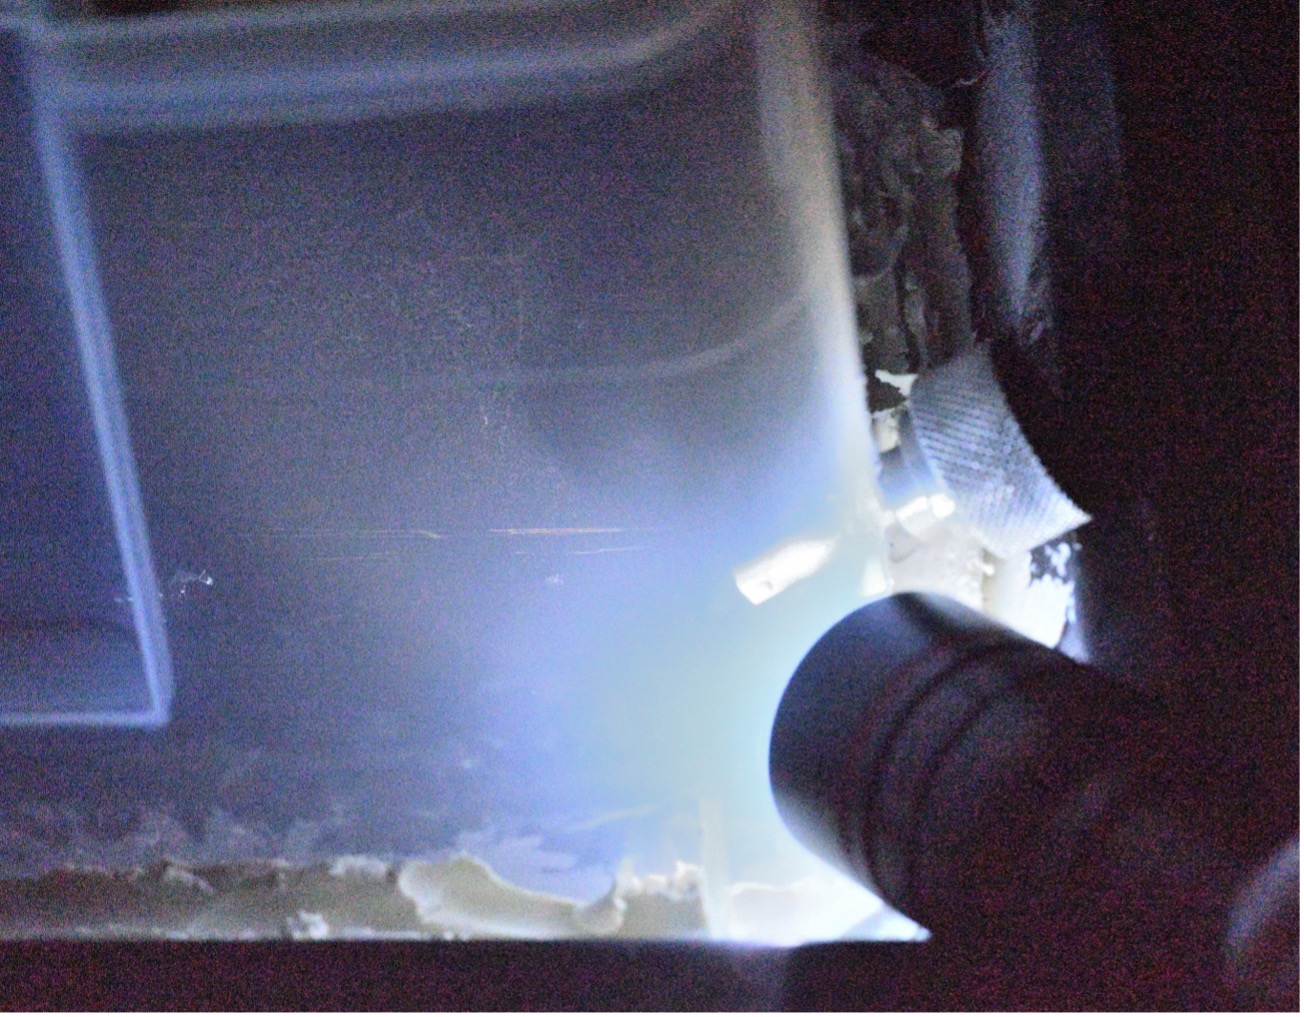
\includegraphics[width=\textwidth, trim={0 100pt 0 300pt}, clip]{Taschenlampe}
	\captionof{figure}[Taschenlampe (rechts), das radioaktive Präparat darüber. Im Hintergrund Teilchenspuren. -- Quelle: Autor.]{Taschenlampe (rechts), das radioaktive Präparat darüber. Im Hintergrund Teilchenspuren.}
	\label{fig:taschenlampe}
	\end{minipage} \\
	
	\vskip 1em
		
	\begin{minipage}[t]{0.31\textwidth}
	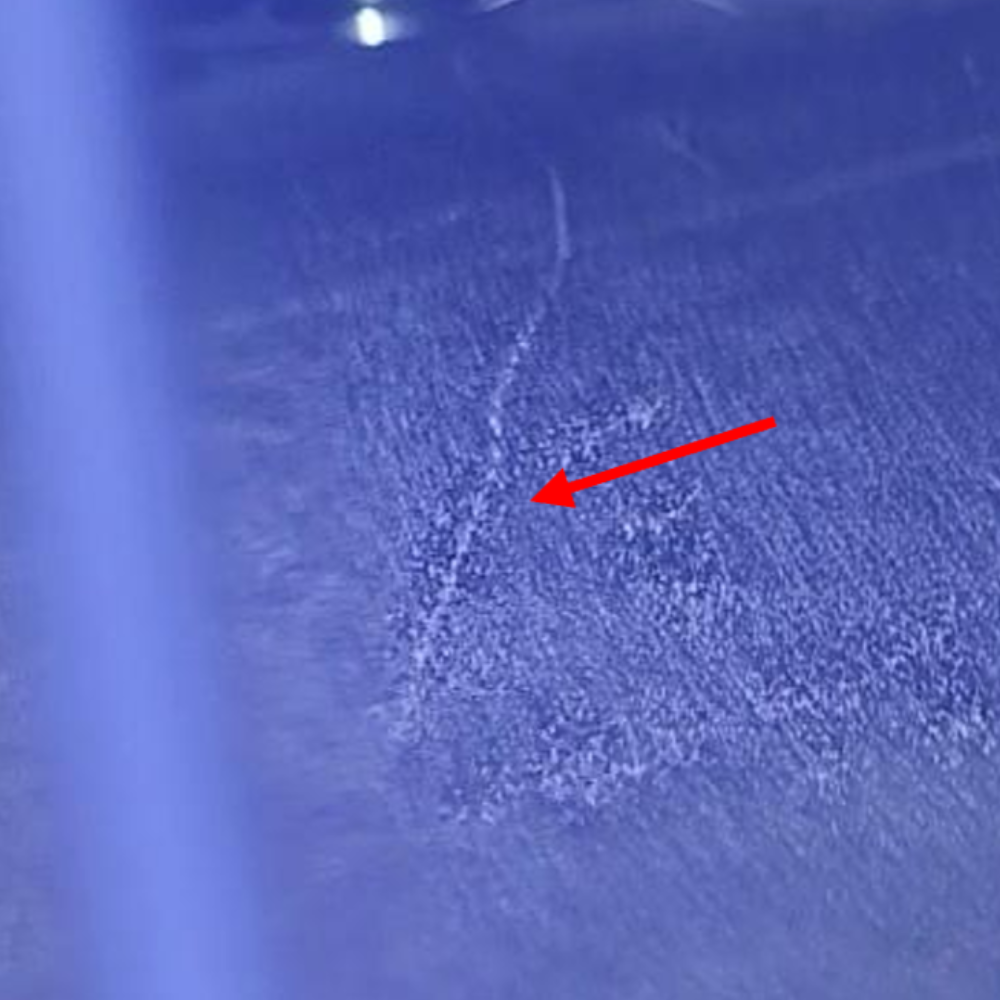
\includegraphics[width=\textwidth, valign=t]{Myon_scaled}
	\captionof{figure}[Geradlinige und deutliche Spur eines Myons. -- Quelle: Autor.]{Geradlinige und deutliche Spur eines Myons.}
	\label{fig:myon}
	\end{minipage} \hfill	
	\begin{minipage}[t]{0.31\textwidth}
	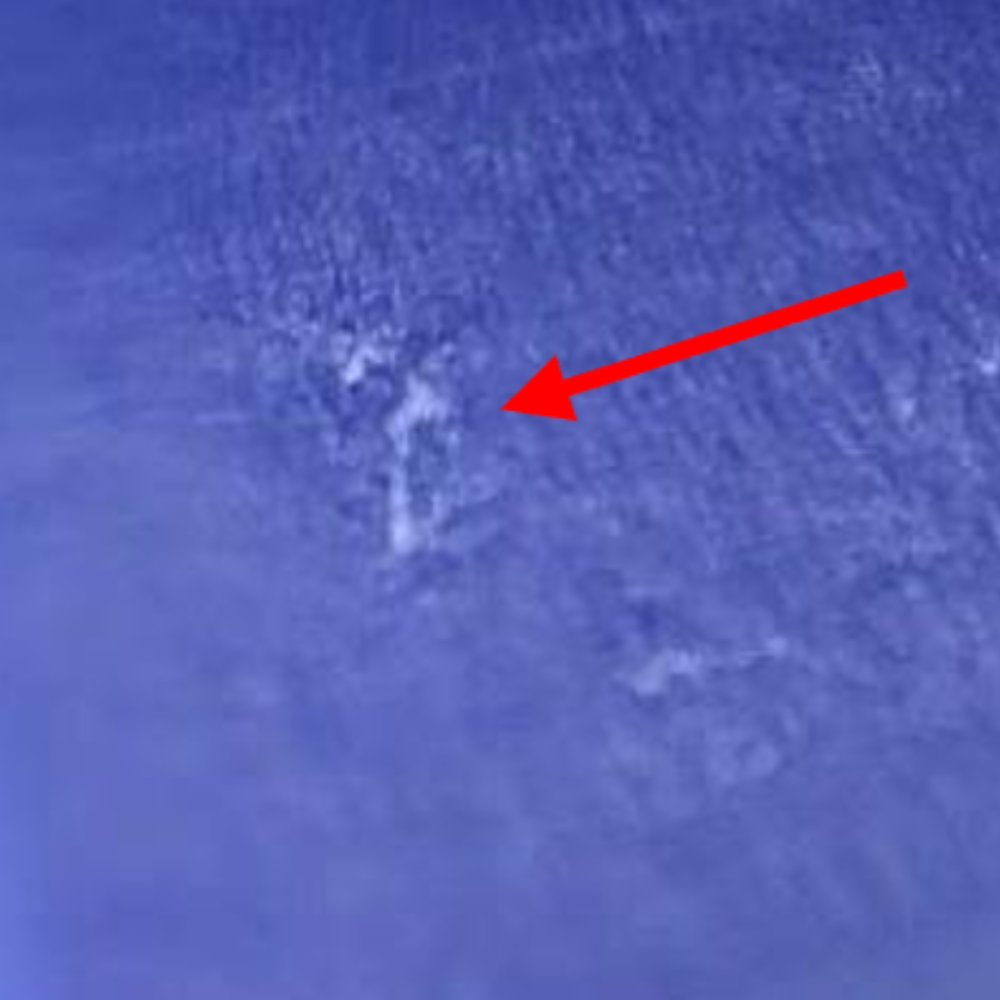
\includegraphics[width=\textwidth, valign=t]{Alpha_scaled}
	\captionof{figure}[Kurze, deutliche Spur eines $\alpha$-Teilchens. -- Quelle: Autor.]{Kurze, deutliche Spur eines $\alpha$-Teilchens.}
	\label{fig:alpha}
	\end{minipage} \hfill
	\begin{minipage}[t]{0.31\textwidth}
	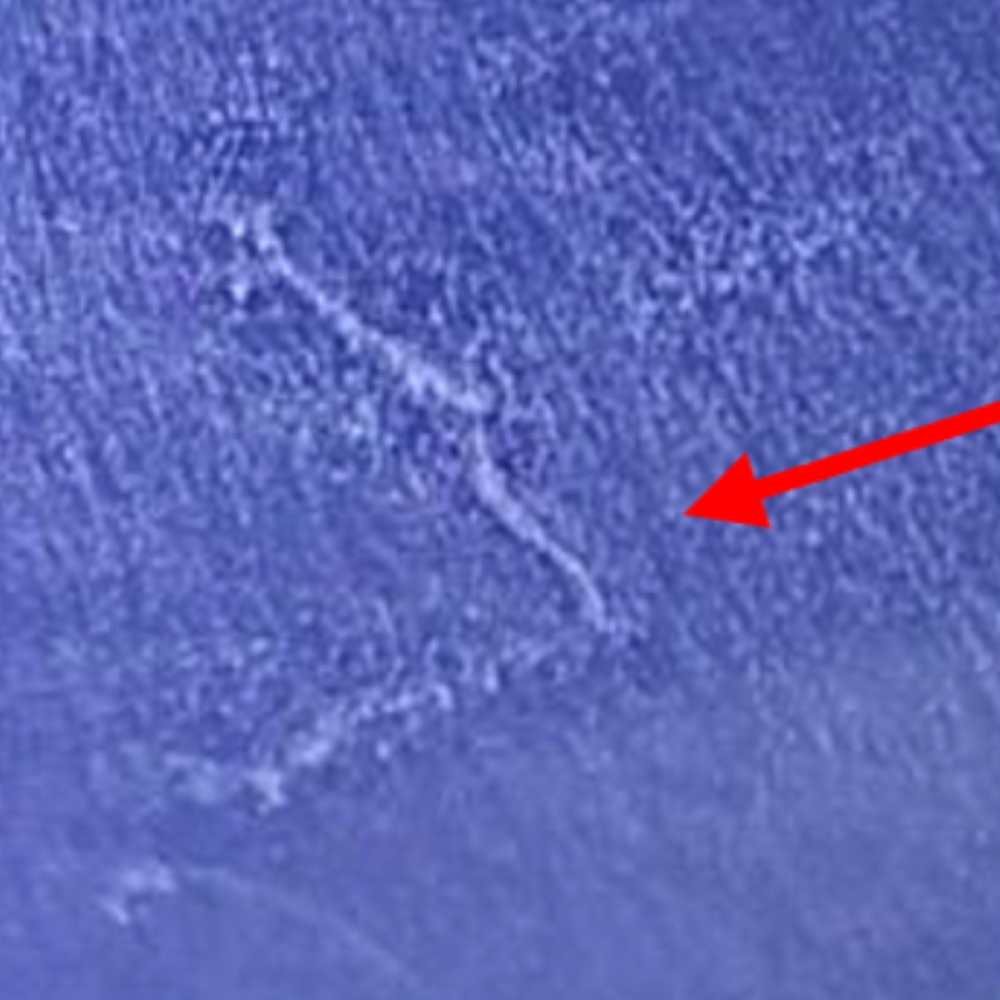
\includegraphics[width=\textwidth, valign=t]{Knick_scaled}
	\captionof{figure}[Teilchenspur mit \glqq Knick\grqq. - Quelle: Autor.]{Teilchenspur mit \glqq Knick\grqq.}
	\label{fig:knick}
	\end{minipage}

\end{table} 
\newpage

	\begin{minipage}[t]{.48\textwidth}
		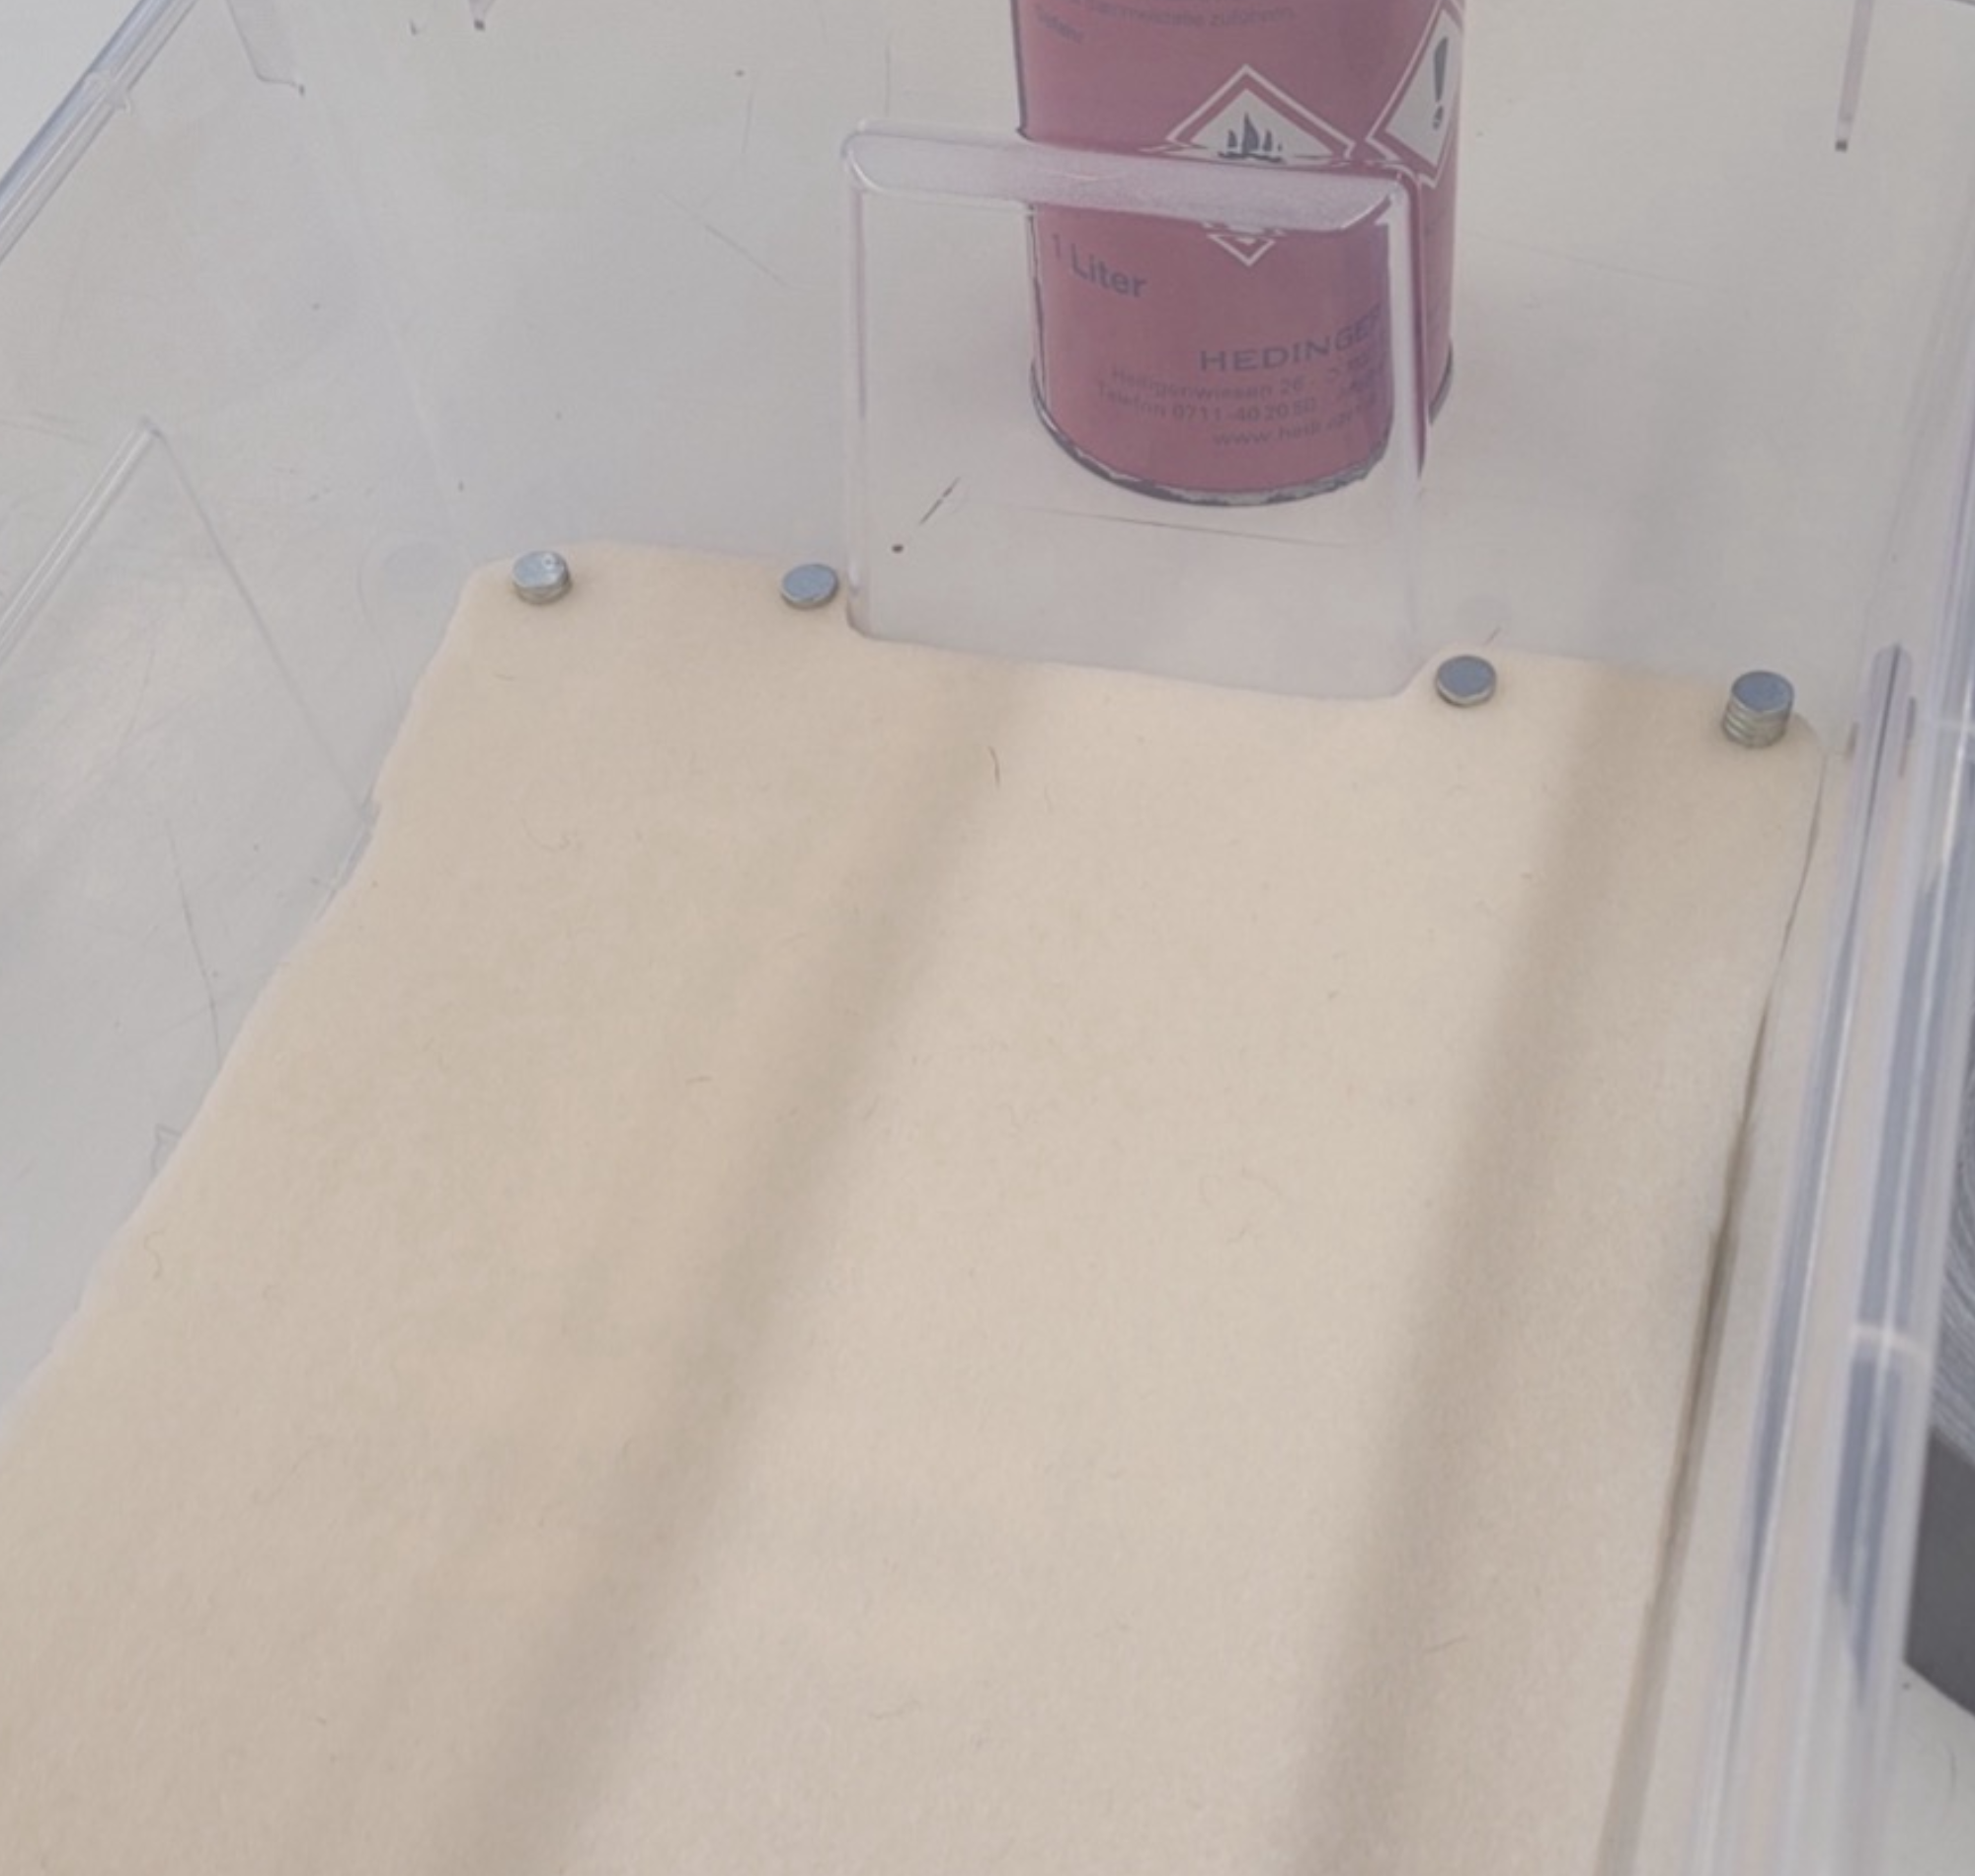
\includegraphics[width=\textwidth]{Abbildung8_scaled}
		\captionof{figure}[Box SAMLA mit Filz und Magneten. -- Quelle: Autor.]{Box SAMLA mit Filz und Magneten.}
		\label{fig:samla}
	\end{minipage} \hfill
	\begin{minipage}[t]{.48\textwidth}
		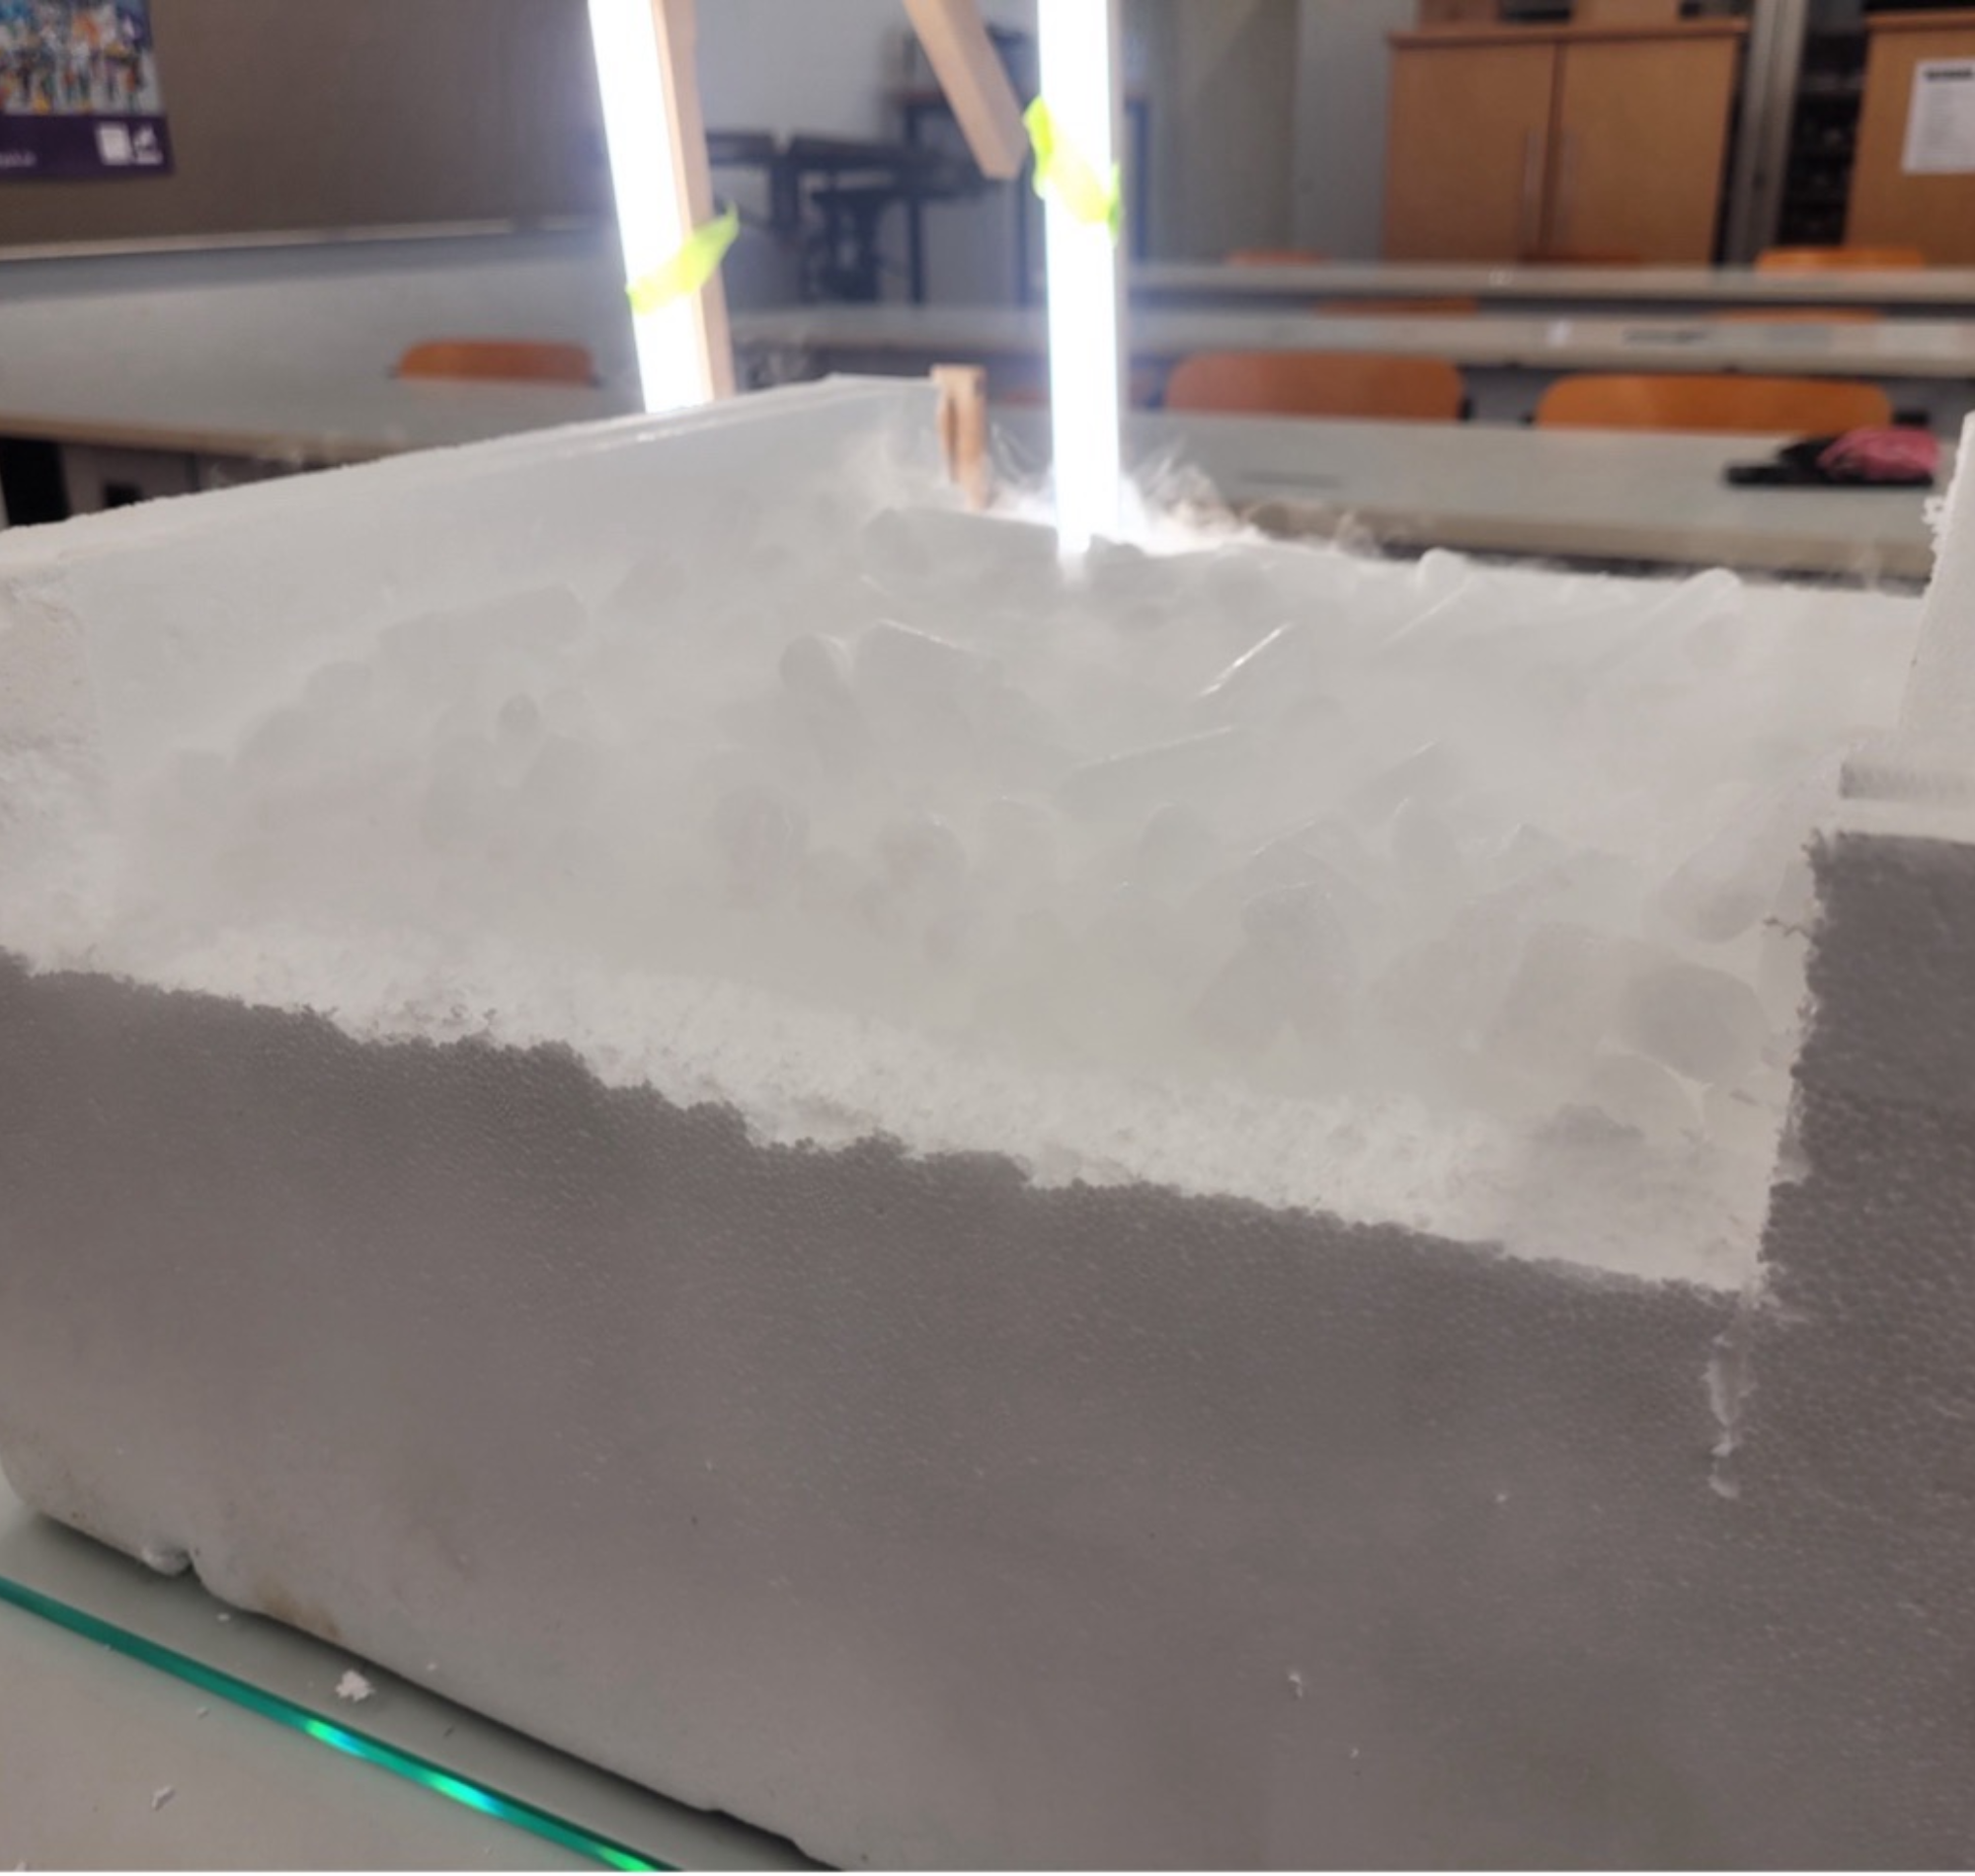
\includegraphics[width=\textwidth]{Abbildung9_scaled}
		\captionof{figure}[Präparierte Styroporkiste mit Trockeneis. -- Quelle: Autor.]{Präparierte Styroporkiste mit Trockeneis.}
		\label{fig:trockeneis}	
	\end{minipage} \\
	
\vskip 1em	
	
	\begin{minipage}[t]{.48\textwidth}
		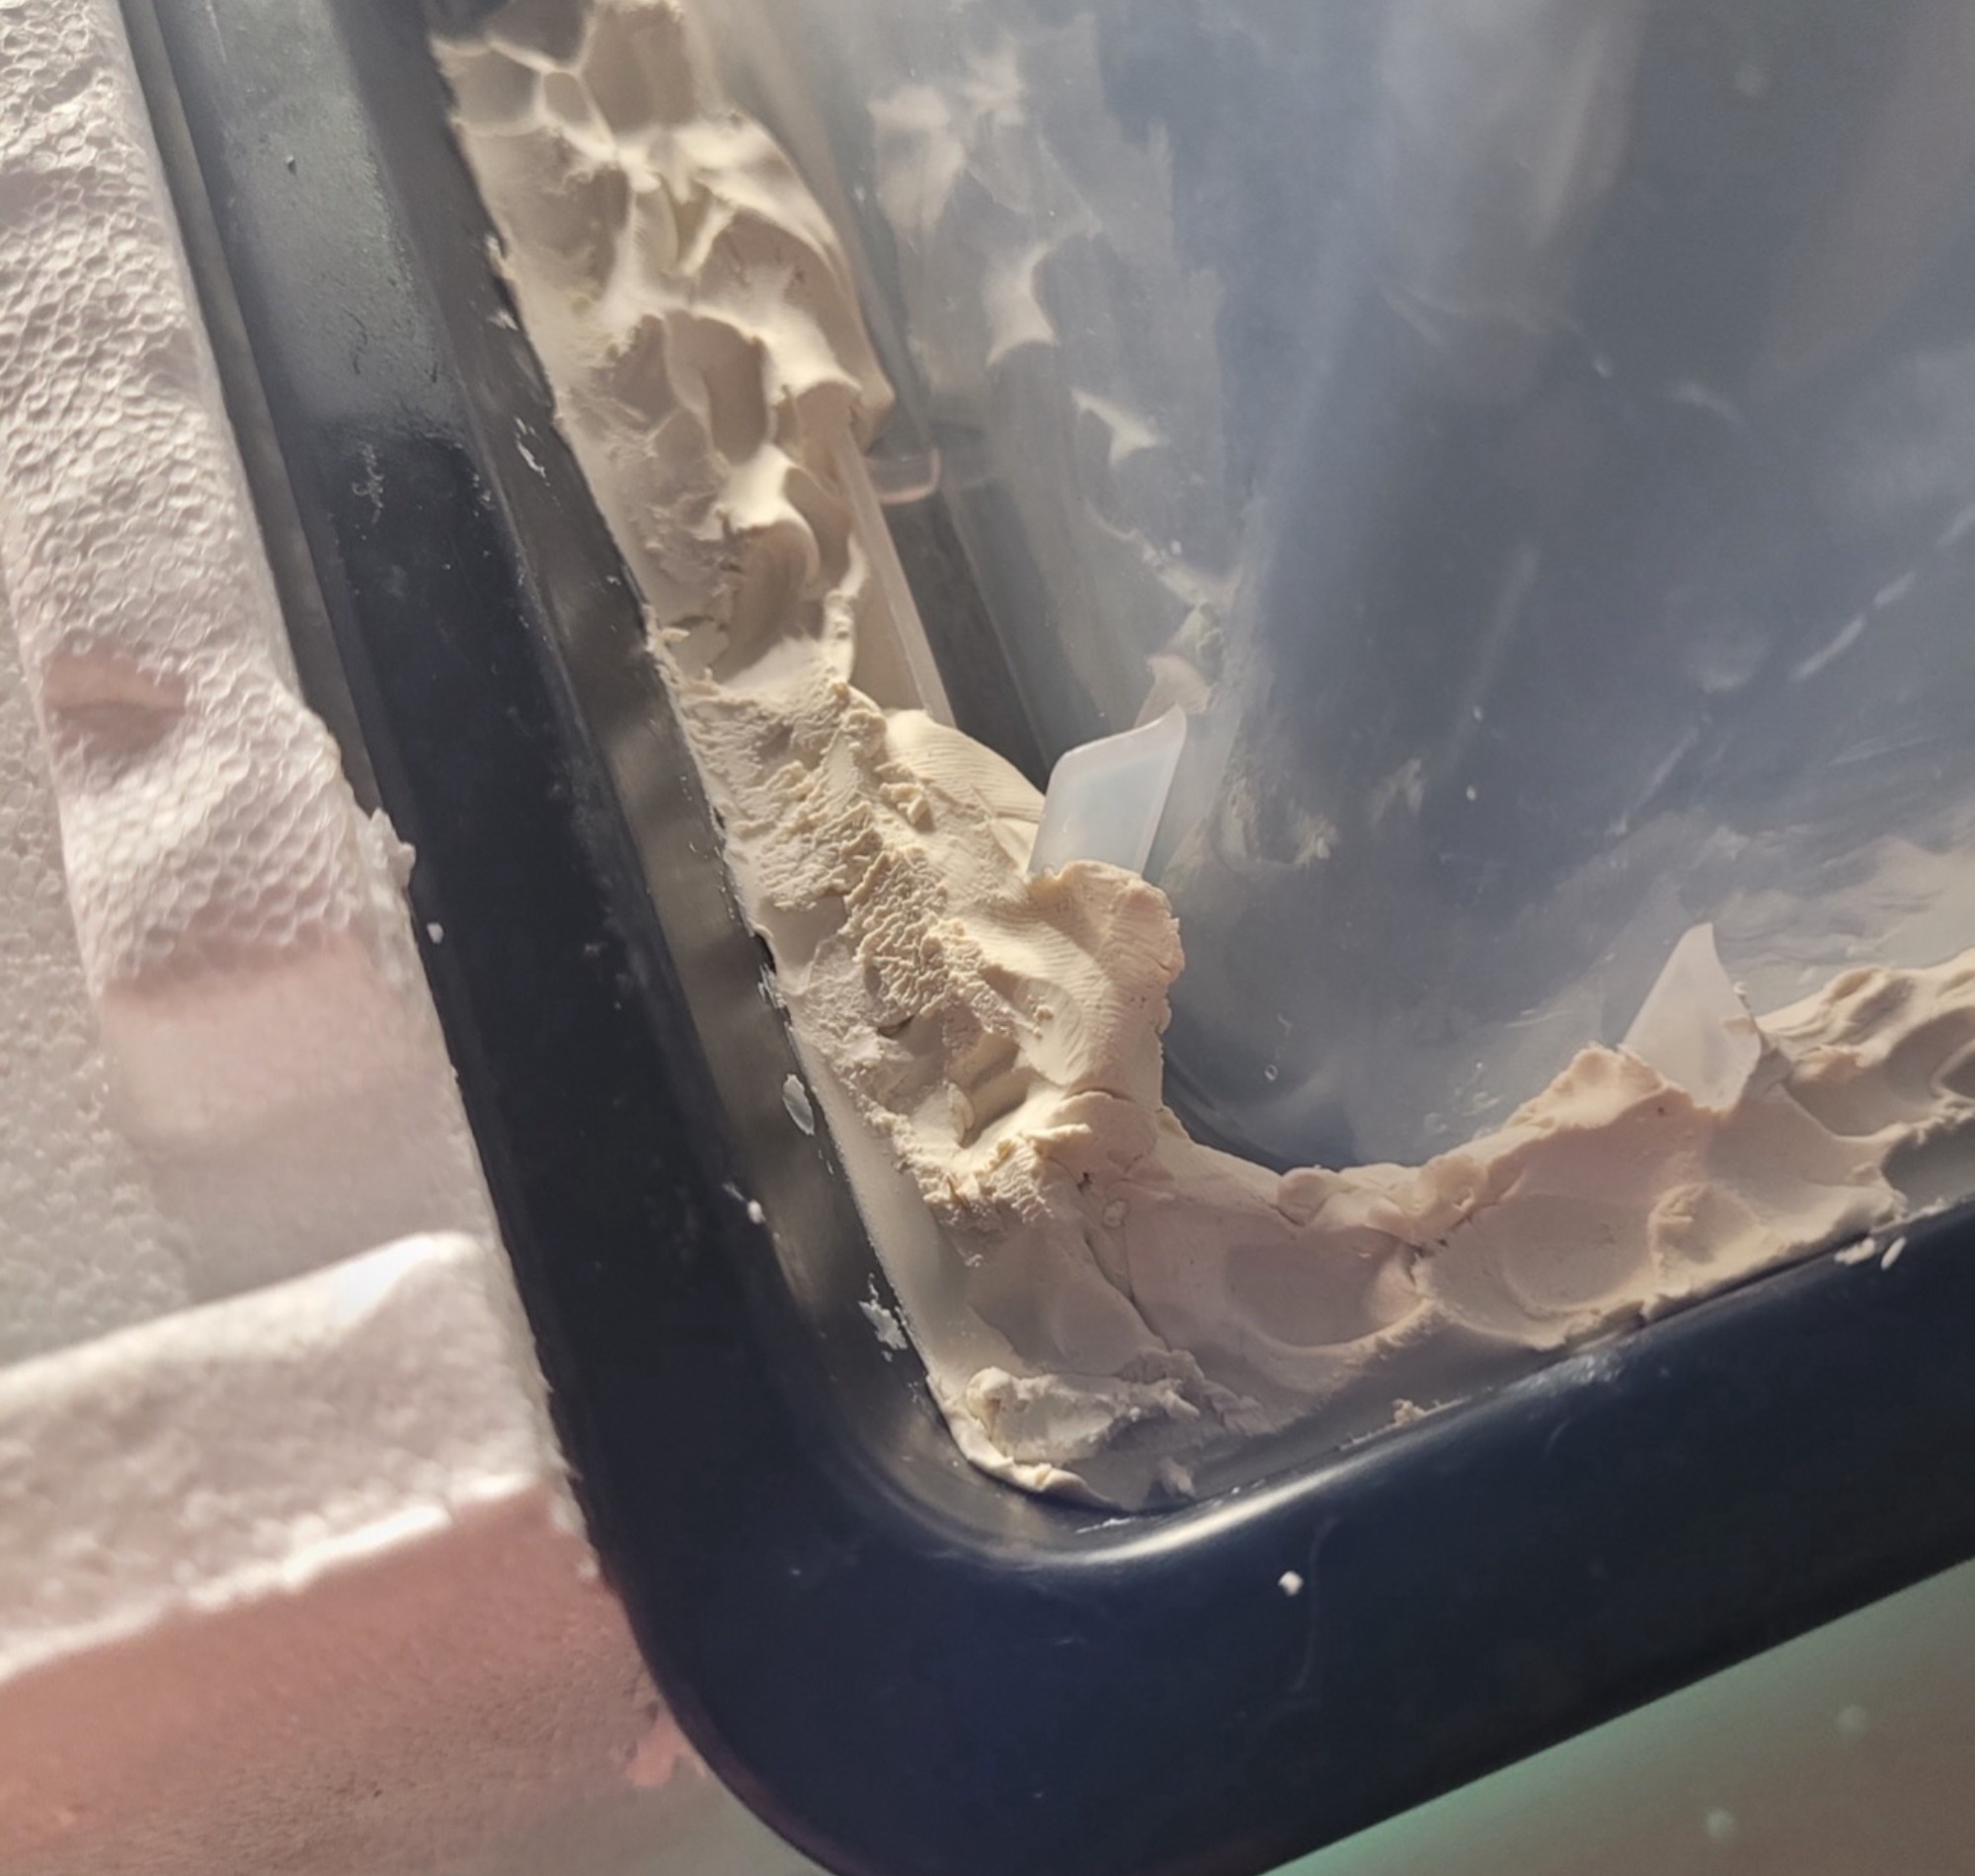
\includegraphics[width=\textwidth]{Abbildung10_scaled}
		\captionof{figure}[Abdichtung mit Plastilin, im Hintergrund das Backblech auf Trockeneis. -- Quelle: Autor.]{Abdichtung mit Plastilin, im Hintergrund das Backblech auf Trockeneis.}
		\label{fig:abdichtung}
	\end{minipage}\hfill
	\begin{minipage}[t]{.48\textwidth}
		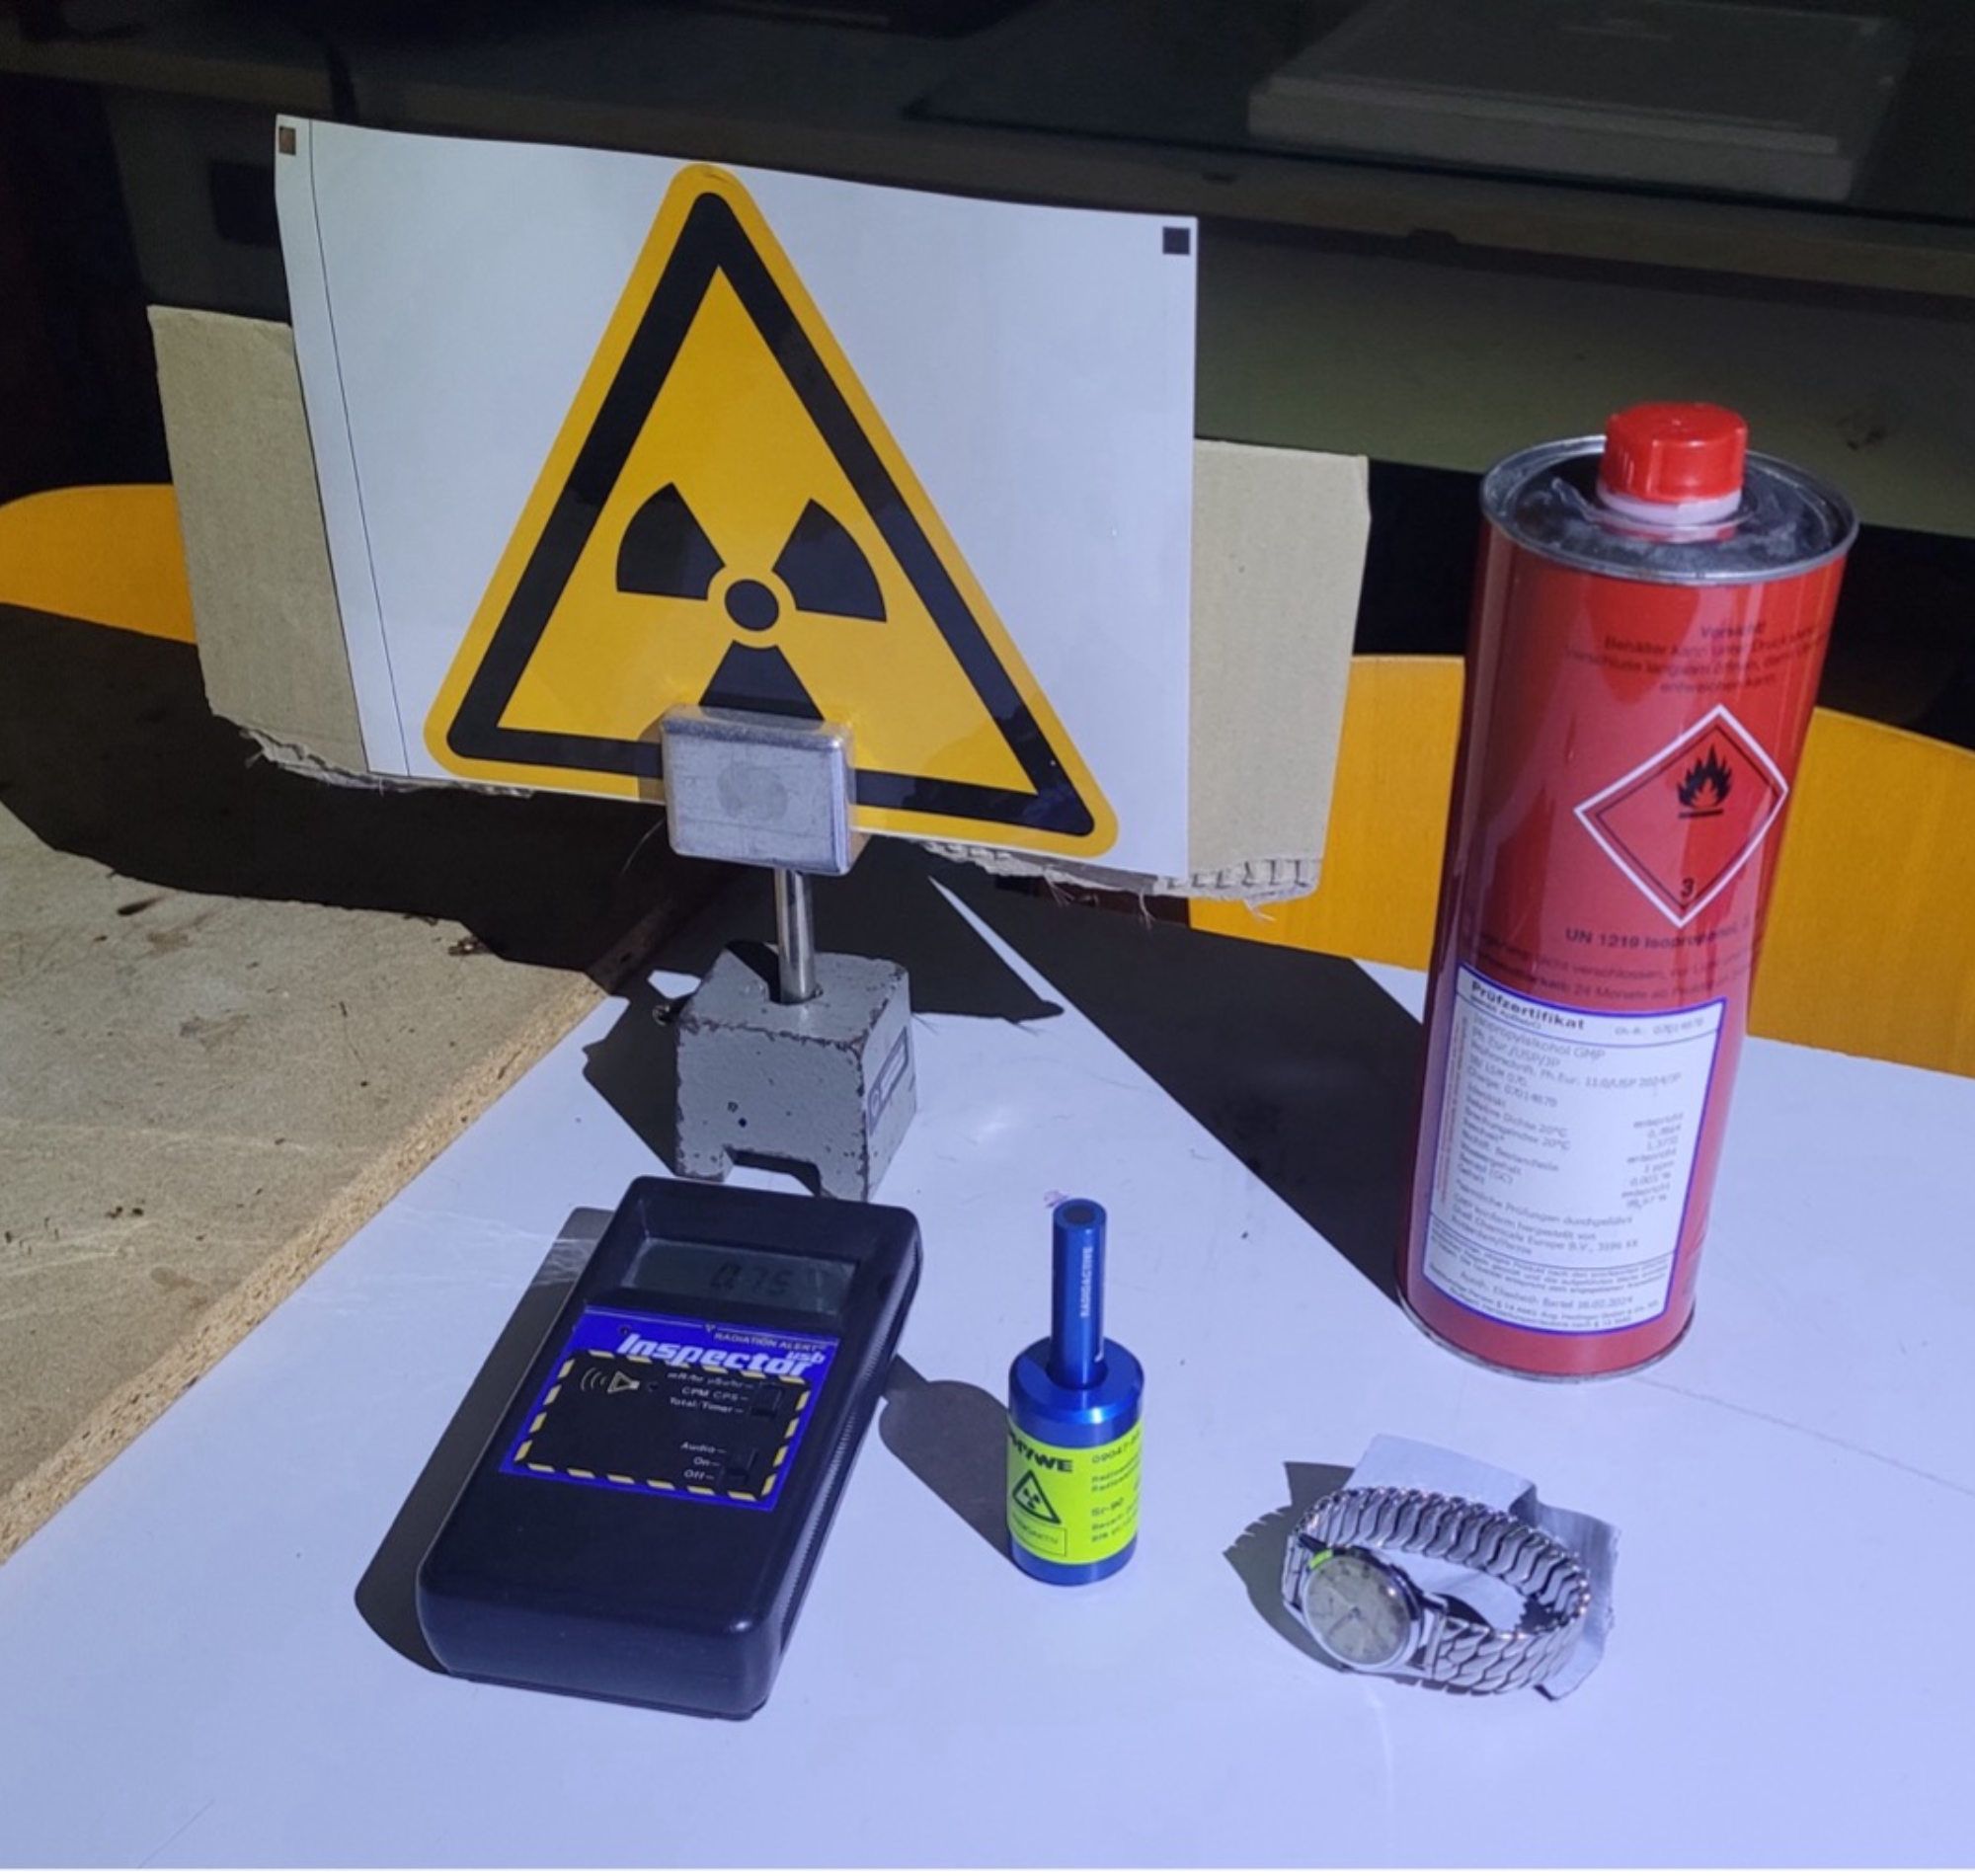
\includegraphics[width=\textwidth]{Abbildung11_scaled}
		\captionof{figure}[Radioaktive Präparate mit Warnschild und Geigerzähler. -- Quelle: Autor.]{Radioaktive Präparate mit Warnschild und Geigerzähler.}
		\label{fig:radiosafety}
	\end{minipage}
	
\newpage

\section{DER ICECUBE NEUTRINO-DETEKTOR} \label{sec:3}
\subsection{Aufbau, Lage und Funktionsweise} \label{ssec:31}

Wie man in \figref{fig:icaufbau} sehen kann, ist der IceCube Neutrino-Detektor ein $\qty{1}{\kilo\meter^3}$ großer Detektor im antarktischen Eis nahe der Amundsen-Scott South Pole Station \cite{UniWisconsin–Madison}. Dabei sind auf einem $\qty{1}{\kilo\meter^2}$ großen hexagonalen Grundriss 86 sog. Strings orthogonal zur Grundfläche ins Eis geschmolzen. Sie haben eine Länge von circa $\qty{2,5}{\kilo\meter}$ und beginnen an der Oberfläche des Eises. $\qty{1450}{\meter}$ unter der Eisoberfläche beginnt eine $\qty{1}{\kilo\meter}$ lange Strecke, an der im Abstand von $\qty{17}{\meter}$ 60 sog. DOMs (Digital Optical Modules) befestigt sind, die die Messergebnisse liefern. Von diesen 5160 DOMs werden die Signale dann in das IceCube Laboratory geleitet, die die Daten verarbeiten und weitersenden \cite{UniWisconsin–Madison}.
\begin{figure}[b!]
\centering
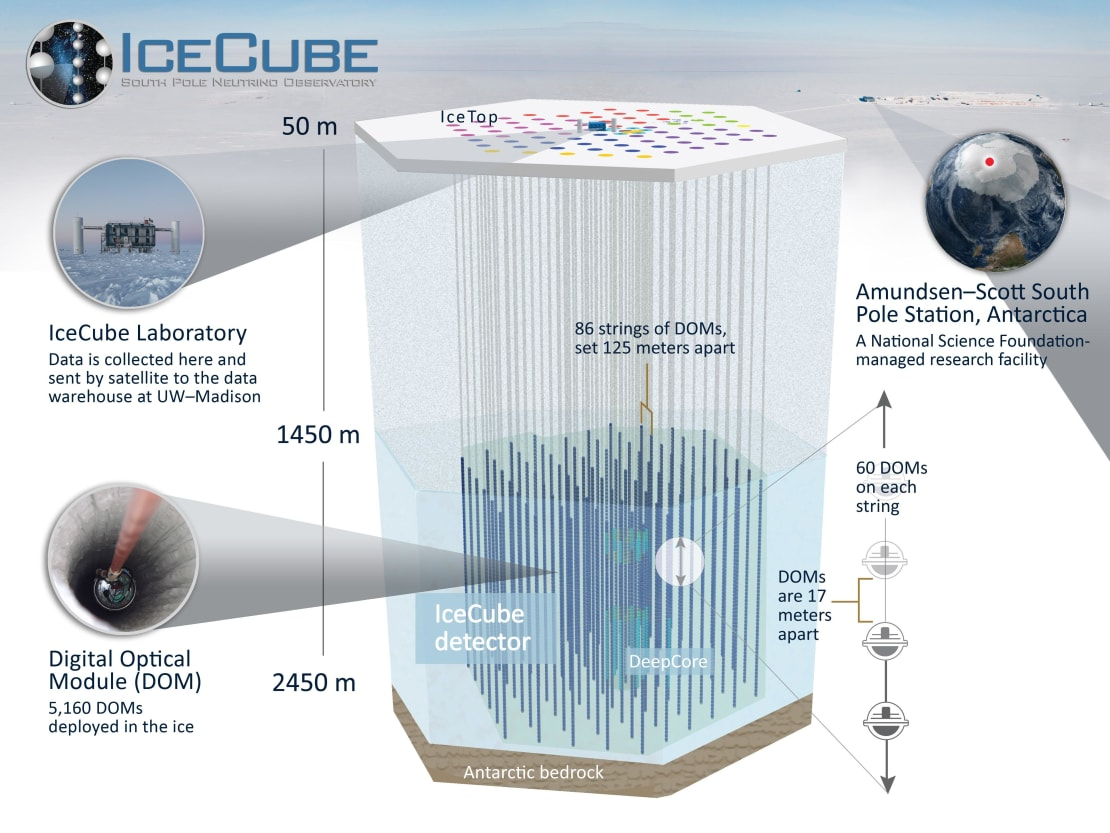
\includegraphics[width=0.8\textwidth]{IceCube}
\caption[Aufbau des IceCube Neutrino-Detektors. -- Quelle: {\cite{UniWisconsin–Madison}}.]{Aufbau des IceCube Neutrino-Detektors.}
\label{fig:icaufbau}
\end{figure}
Um die Funktionsweise des Detektors zu verstehen, wird nochmals auf \cref{ssec:24} zurückgegriffen. Interagiert ein Neutrino mit Eis, so werden elektrisch geladene Sekundärteilchen produziert \cite{UniWisconsin–Madison}. Diese Sekundärteilchen können sich mit sehr hohen Energien durch das Eis bewegen und sind dabei schneller als Licht im Eis, was zur Cherenkov-Strahlung führt \cite[14]{HaMinh2025}. Dieser Lichtkegel wird von den DOMs detektiert und lässt Rückschlüsse auf Art, Energie und Geschwindigkeit des Sekundärteilchens, und damit auch des Neutrinos, ziehen \cite[15]{HaMinh2025}. 
\begin{figure}[b!]
\centering
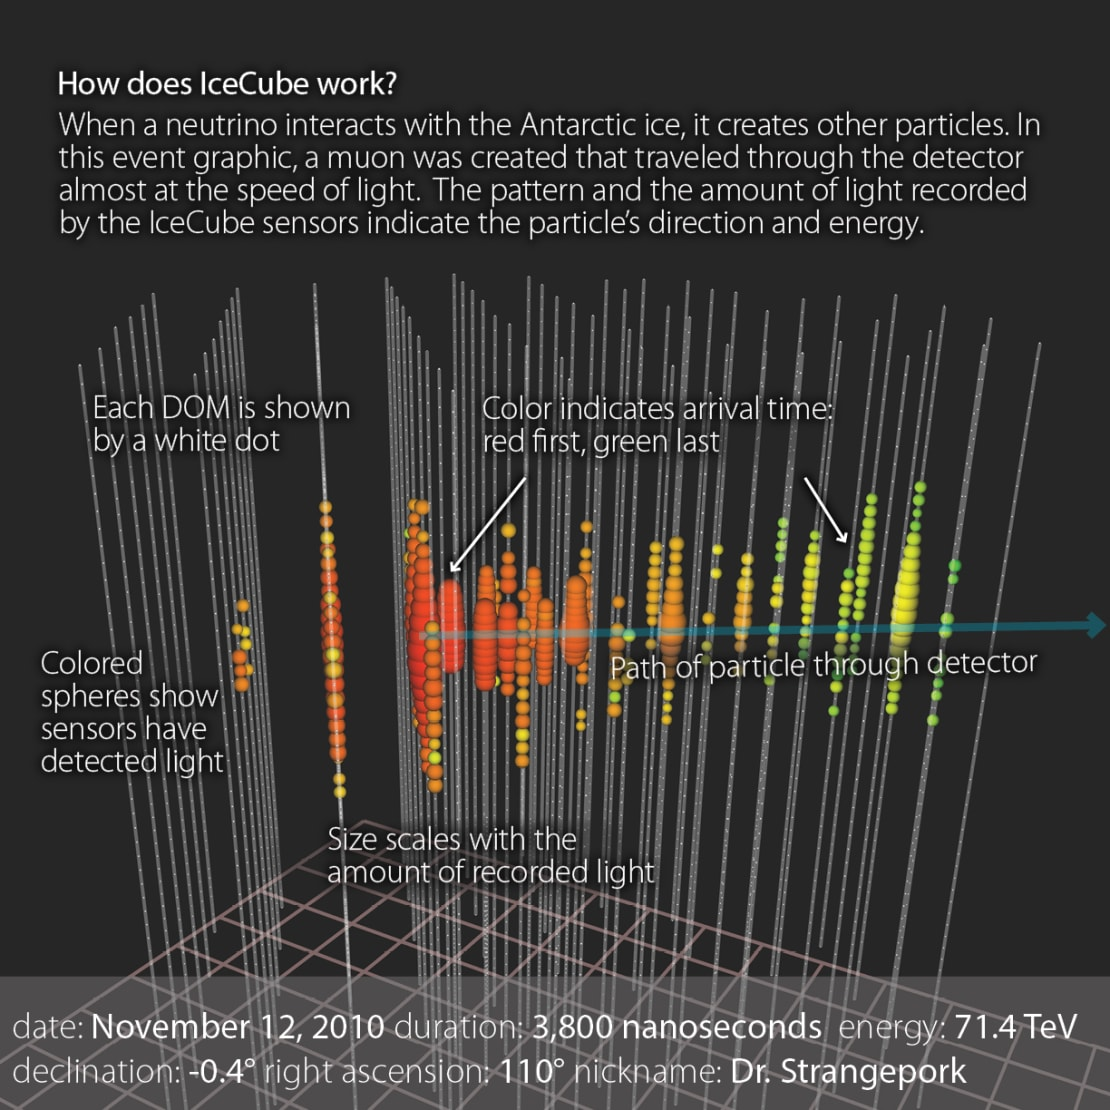
\includegraphics[width=0.8\textwidth]{HowDoesIceCubeWork}
\caption[Funktionsweise des IceCube Detektors anhand der grafischen Darstellung eines Events. -- Quelle: {\cite{UniWisconsin–Madison}}]{Funktionsweise des IceCube Detektors anhand der grafischen Darstellung eines Events.}
\label{fig:icfunktion}
\end{figure}

\subsection{Wissenschaftliche Erfolge} \label{ssec:32}

Der Aufbau des Detektors kostete 279 Millionen US-Dollar \cite{UniWisconsin–Madison}, doch warum zahlt man so viel Geld? Zwei Jahre nach Inbetriebnahme gab es einen ersten Erfolg: Der Detektor nahm in 662 Tagen Betriebszeit 28 Events (vgl. \figref{fig:icfunktion}) von Neutrinos auf -- deutlich mehr als die erwartete atmosphärische Hintergrundstrahlung von $\num{10,6}_{-3,6}^{+5,0}$ Events \cite{IceCubeCollaboration2013}. Es wurden also Neutrinos aus dem Weltraum detektiert. Doch zu diesem Zeitpunkt konnte man die Richtung der Neutrino-Events noch nicht eindeutig zuordnen. Im Laufe der Jahre konnten allerdings durch den IceCube Detektor der Blazar TXS 0506+056 \cite{Aartsen2018} und die aktive Galaxie NGC 1068 \cite{Abbasi2022} als punktförmige Hochenergie-Neutrino-Quellen identifiziert werden. Während auf dieser Strecke die meisten Teleskope versagen, sind Gamma-Teleskope zwar in der Lage, aus Distanzen im Bereich von $\qty{14}{\mega\parsec} \approx \qty{47e6}{\lightyear}$ bzw. $\qty{2,97e12}{\astronomicalunit}$ (wie im Fall von NGC 1068) Daten zu empfangen. Jedoch interagieren Photonen, also auch Gamma-Strahlen, leichter mit anderen Teilchen, was Neutrinos zur zuverlässigeren Informationsquelle macht \cite{Abbasi2022}. Die Richtung von Photonen kann durch die elektromagnetische Wechselwirkung beeinflusst werden, wodurch nicht mehr klar ist, aus welcher Richtung das Photon stammt. Neutrinos hingegen wechselwirken nicht elektromagnetisch, was auf immer größer werdenden Distanzen einen gravierenden Unterschied macht. Die Neutrino-Astronomie ermöglicht es nicht zuletzt, Informationen aus Bereichen des Universums zu erlangen, aus denen Photonen keine brauchbaren Informationen mehr liefern \cite{DESD}.

\subsection{Zukunft des IceCube Neutrino-Detektors} \label{ssec:33}

Nach mehr als zehn Jahren Betriebszeit sind Planungen vorangeschritten, wie man den IceCube Neutrino-Detektor noch effizienter und besser gestalten kann (vgl. \figref{fig:detektorausbau}). Bis zum Jahre 2032 will man das Volumen des Detektors um den Faktor acht erweitern und die pro Jahr detektierten Neutrino-Events sogar auf eine Million erhöhen \cite{DESD}. Es wird geplant, den Kern des Detektors mit mehr DOMs auszustatten und nahe der Eisoberfläche auf 500 Quadratkilometern Radiodetektoren zu errichten, um die Messgenauigkeit zu erhöhen \cite{DESD}. Auf der Eisoberfläche selbst werden zusätzlich neue Messinstrumente angebracht. Schließlich soll auch Maschinelles Lernen zum Auswerten der vielen Events genutzt werden, um in unerreichter Geschwindigkeit und hoher Präzision Neutrino-Events aus den Messdaten herauszufiltern \cite{DESD}.
\begin{figure}[H]
\centering
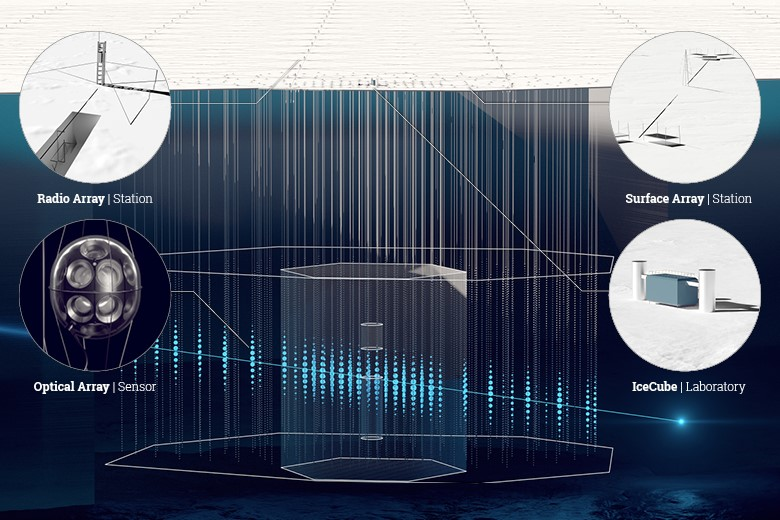
\includegraphics[width=0.8\textwidth]{Detektorausbau}
\caption[Visualisierung des Detektorausbaus zu IceCube-Gen2. Das kleine Hexagon in der Mitte repräsentiert den bisherigen IceCube Detektor, während das größere Hexagon die Grundfläche von IceCube-Gen2 erahnen lässt. \copyright DESY, Science Communication Lab. -- Quelle: {\cite{DESD}}]{Visualisierung des Detektorausbaus zu IceCube-Gen2. Das kleine Hexagon in der Mitte repräsentiert den bisherigen IceCube Detektor, während das größere Hexagon die Grundfläche von IceCube-Gen2 erahnen lässt.}
\label{fig:detektorausbau}
\end{figure}


\section{FAZIT} \label{sec:4}

Neutrinos konnten die Wissenschaft seit ihrer Postulierung im Jahre 1930 begeistern. Bis heute spielen sie eine wichtige Rolle bei der Erforschung von Teilchenprozessen wie dem $\upbeta$-Zerfall, ermöglichen einen Blick ins Innere der Sonne und bereichern die Astrophysik außerdem mit einem Blick in bislang unbekanntes Terrain. Dabei zeigen diese geheimnisvollen Geisterteilchen, dass Wissenschaft stets ein Diskurs ist, in dem man auch irren darf. Ob es Pontecorvo mit dem Chlortank oder Pauli selbst war, der den Unterschied von Neutron und Neutrino nicht erkannte, durch Diskurs und gute Zusammenarbeit strebt man stets nach neuen Erkenntnissen. \par
Nur durch die weltweite Kollaboration von vielen Wissenschaftlerinnen und Wissenschaftlern konnte in dieser Wissenschaftspropädeutischen Arbeit eine Teilchenart untersucht werden, die es vorzieht, unentdeckt zu bleiben. Winzig klein, fast masselos, und dennoch mit gravierendem Effekt: Ohne Neutrinos geht es, spätestens seit dem Zwiespalt mit dem $\upbeta^-$-Zerfall aus \cref{ssec:21}, nicht mehr. Elementarteilchen wie das Neutrino lassen sich dabei nur schwer nachweisen. Wie in \cref{ssec:25} experimentell untersucht, nutzt man deshalb Spuren von Sekundärteilchen, die von den nachzuweisenden Teilchen erzeugt werden. Nach diesem Prinzip lassen sich mithilfe von großen Experimenten wie dem IceCube Neutrino-Detektor und der Cherenkov-Strahlung die Neutrinos besser denn je erforschen. \par 
Es bleibt abzuwarten, inwieweit mit IceCube-Gen2 weitere Forschungserkenntnisse gewonnen werden können. Ob es möglich sein wird, neue Galaxien zu entdeckten, gar außerirdisches Leben? Vielleicht kann IceCube-Gen2 eine weitere Supernova einfangen, und uns damit mehr über diese kosmischen Explosionen verraten. \par
Spannend bleibt auch die Diskussion um Dirac- und Majorana-Neutrinos. Es wird sich zeigen, was in den nächsten Jahren in der Neutrino-Forschung passiert. Klar ist: Die Wissenschaft ist heute wohl interessierter denn je an den Geisterteilchen. Mit IceCube-Gen2 wird ein großer Forschritt erzielt, doch auf der ganzen Welt entstehen Detektoren wie das Jiangmen Underground Neutrino Observatory (JUNO) in China \cite{UniJohannesGutenbergMainz2025, JUNO2025} oder das Ausbauprojekt \glqq High-Luminosity LHC\grqq \ des LHC in Cern \cite{UniBonn2025}. Die Datenmenge der Geisterteilchen sollte also zunehmen, wodurch Neutrinos wohl immer besser verstanden werden können.

\nocite{Hu2017}

\newpage

\section{ANHANG} \label{sec:5}
\printbibliography[title=Literaturverzeichnis]

\newpage

\listoffigures

\newpage

\listoftables

\end{document}